% cd /host-rootfs/storage/emulated/0/Documents/documents/latex/1920/; pdflatex dll-05-31-2019.tex

% cd /storage/emulated/0/Documents/documents/latex/1920/Grade-10/1st/05-31-2019/; pdflatex dll-05-31-2019.tex; termux-open dll-05-31-2019.pdf; rm *.csv

% cd /host-rootfs/storage/emulated/0/Documents/documents/latex/1819/grade10/lesson; convert -density 600 new-dll-05-31-2019.pdf -quality 100 new-dll-05-31-2019.png

\documentclass[11pt]{article}
\usepackage[pdftex]{graphicx}
\usepackage[legalpaper, landscape, right=0.5in,  left=1.5in, top=0.5in, bottom=0.5in]{geometry}

\usepackage{booktabs}
\usepackage{bm}
\usepackage{longtable}
\usepackage{fourier} % always fourier before amssymb
\usepackage{array} 
\usepackage{datatool}
\usepackage{xcolor}
\usepackage{anyfontsize}
\usepackage{enumitem}
\usepackage{multicol}
\usepackage{amsmath, makecell}
\usepackage{tabularx} 
\usepackage{gensymb}
\usepackage{wasysym} %for checked symbol 
\usepackage{multirow}
\usepackage{graphicx, tipa}
\usepackage{tikz}
\usetikzlibrary{angles,quotes}
\usepackage{pgfplots} 
\usetikzlibrary{calc}
\pgfplotsset{compat=newest}
\usetikzlibrary{arrows.meta}
\usetikzlibrary{intersections}
\usetikzlibrary{decorations.pathreplacing}
\usepackage{flafter}
%\usepackage{fourier} 
\usepackage{amsmath,amssymb,cancel,units}
\usepackage{microtype} % nicer output 
\usepackage{hfoldsty} % nicer output 
\usepackage{fixltx2e} 
\usepackage{mathptmx}
\usepackage{numprint}
\usepackage[T1]{fontenc}
\usepackage[utf8]{inputenc} 
\usepackage{stackengine} %to define \pesos 
\usepackage{lmodern} %scalable font
\usepackage{booktabs}
\usepackage{array}


\pagenumbering{gobble}
%\linespread{0.9}
\newcommand{\vspce}{\vspace{0.75ex}}

\newcommand{\hspce}{\hspace{0.5em}}

\newcommand{\blank}{\underline{\hspace{2em}}}%{\rule{1em}{0.15ex}}

\newcommand{\arc}[1]{{% 
\setbox9=\hbox{#1}% 
\ooalign{\resizebox{\wd9}{\height}{\texttoptiebar{\phantom{A}}}\cr#1}}}


\newcommand\pesos{\stackengine{-1.4ex}{P}{\stackengine{-1.25ex}{$-$}{$-$}{O}{c}{F}{F}{S}}{O}{c}{F}{T}{S}} 


\renewcommand\theadalign{bc} 

\renewcommand\theadfont{\bfseries} 

\renewcommand\theadgape{\Gape[4pt]} 

\renewcommand\cellgape{\Gape[4pt]} 

\pagenumbering{gobble}

\newcolumntype{Y}{>{\centering\arraybackslash}X} %for tabularx

\newcolumntype{R}{>{\raggedleft\arraybackslash}X} %for tabularx

\newcolumntype{Z}{>{\raggedleft\arraybackslash}X} %for tabularx

\newcolumntype{L}{>{\raggedright\arraybackslash}X} %for tabularx

\newcolumntype{A}[1]{>{\raggedright\arraybackslash}p{#1}} %for longtable LEFT

\newcolumntype{C}[1]{>{\centering\arraybackslash}p{#1}} %for longtable CENTER

\newcolumntype{B}[1]{>{\raggedleft\arraybackslash}p{#1}} %for longtable RIGHT 
 
\renewcommand{\tabularxcolumn}[1]{>{\small}m{#1}}

\newcolumntype{N}[1]{>{\raggedleft}p{#1}} %for tabular left 

\newcolumntype{M}[1]{>{\raggedright\arraybackslash}p{#1}} %for tabular right 

\newcommand{\myaxis}{xticklabels={}, 
yticklabels={}, 
ymin=-10, ymax=10,
xmin=-10, xmax=10,
axis lines = center, 
inner axis line style={Latex-Latex,very thick}, 
grid=both,
minor tick num=4, 
tick align=inside} % grid without labels, origin at the center, 10 units from origin

\newcommand{\axisfive}{xticklabels={}, 
yticklabels={}, 
ymin=-5, ymax=5,
xmin=-5, xmax=5,
axis lines = center, 
inner axis line style={Latex-Latex,very thick}, 
grid=both,
minor tick num=1, 
tick align=inside} % grid with labels, origin at the center, 5 units from origin 

\newcommand \redcheck {{\color{red}\checkmark}}

 

\setlength{\extrarowheight}{2pt} 

\def \Grade {10}

\def \Quarter {2nd}

\def \School {Sauyo High School }

\def \Teacher {Mr. Jonathan R. Bacolod, LPT }

\def \Subject {Mathematics }

\def \Checker {DR. LORETO R.  DOMINGO \\
Head, Mathematics Department }

\begin{filecontents*}{sections.csv} 
Section
Bohr
Avogadro 
\end{filecontents*}

\DTLloaddb{Section}{sections.csv}

\def \RemedialOne {\DTLforeach*{Section}{\Section=Section}{\Grade--\Section: \blank out of \blank \newline}}

\def \RemedialTwo {\DTLforeach*{Section}{\Section=Section}{\Grade--\Section: \blank \newline}}

\def \Remark {Objectives have
been attained: \blank \newline
Objectives were not attained due to: \underline{\hspace{10em}}}

 


%%%% Edit this section ONLY. 
\def \LessonWeek {September 23 -- 27, 2019}

\def \WeekNum {17}

\def \Content {\multicolumn{4}{c|}{\thead{PATTERNS AND ALGEBRA}}}

\def \ContentStandards {
\multicolumn{4}{l|}{\makecell{
The learner demonstrates understanding of key concepts of sequences, polynomials and polynomial equations. 
}}}

\def \PerformanceStandards {
\multicolumn{4}{l|}{\makecell{
The learner is able to formulate and solve problems involving sequences, polynomials and polynomial equations \\in different disciplines through appropriate and accurate representations
}}}
%%%%%%%%

%%% Don't change this section! 
%\input{LESSONS-TODAY} 

%
% Start the document
\begin{document}


\begin{center}

{
\setlength\arrayrulewidth{2pt}
\begin{tabularx}{\textwidth}{|Y|R|L|R|L|}

\hline

\multirow[c]{3}{15em}{
\begin{tikzpicture}[remember picture, overlay]
\node (deped) at (135:1mm) {
\includegraphics[width=3.5em]{/storage/emulated/0/Documents/documents/latex/1920/deped2.png}};
\end{tikzpicture}
\centering \textbf{\makecell{GRADES 1 to 12 \\ DAILY LESSON LOG}}
}  
& 	
\textbf{School}  & 
\School & 	
\textbf{Grade Level} & 
Grade \Grade 
\\

\cline{2-5}

& \textbf{Teacher} 
& \Teacher 
& \textbf{Learning Area} 
& \Subject \\

\cline{2-5}

& \textbf{Teaching Dates and Time} 
& Week \WeekNum, \LessonWeek 
& \textbf{Quarter} 
& \Quarter \\

\hline

\end{tabularx} 
}


\begin{longtable}{|p{161pt}|p{161pt}|p{161pt}|p{161pt}|p{161pt}|}

\hline

\textbf{I. OBJECTIVES } & 	
\thead{DAY 1}  & 
\thead{DAY 2}  & 	
\thead{DAY 3}  & 
\thead{DAY 4}  \\

\hline

\hspce \textbf{A. Content Standards:}  	
& 
\ContentStandards
\\ 

\hline 

\hspce \textbf{B. Performance Standards:}  	
& 
\PerformanceStandards
\\ 
\hline 

\hspce \textbf{C. Learning Competencies/ \newline Objectives: (Write the LC code for each.) }
&	

% Day 1 Learning Competencies
\if \LessonA1 
\LearningCompetenciesDayA
\fi 
\if \LessonB1 
\LearningCompetenciesDayB
\fi 
\if \LessonC1 
\LearningCompetenciesDayC
\fi 
\if \LessonD1 
\LearningCompetenciesDayD
\fi 

\begin{enumerate}[leftmargin=1em, nolistsep]
\if \LessonA1 
\ObjectivesDayA
\fi
\if \LessonB1 
\ObjectivesDayB
\fi
\if \LessonC1 
\ObjectivesDayC
\fi
\if \LessonD1 
\ObjectivesDayD
\fi
\end{enumerate}

&

% Day 2 Learning Competencies
\if \LessonA2
\LearningCompetenciesDayA
\fi 
\if \LessonB2
\LearningCompetenciesDayB
\fi 
\if \LessonC2
\LearningCompetenciesDayC
\fi 
\if \LessonD2
\LearningCompetenciesDayD
\fi 
 
\begin{enumerate}[leftmargin=1em, nolistsep]
\if \LessonA2 
\ObjectivesDayA
\fi
\if \LessonB2 
\ObjectivesDayB
\fi
\if \LessonC2 
\ObjectivesDayC
\fi
\if \LessonD2 
\ObjectivesDayD
\fi
\end{enumerate}

& 

% Day 3 Learning Competencies
\if \LessonA3
\LearningCompetenciesDayA
\fi 
\if \LessonB3
\LearningCompetenciesDayB
\fi 
\if \LessonC3
\LearningCompetenciesDayC
\fi 
\if \LessonD3
\LearningCompetenciesDayD
\fi 
 
\begin{enumerate}[leftmargin=1em, nolistsep]
\if \LessonA3 
\ObjectivesDayA
\fi
\if \LessonB3 
\ObjectivesDayB
\fi
\if \LessonC3 
\ObjectivesDayC
\fi
\if \LessonD3 
\ObjectivesDayD
\fi
\end{enumerate}

&

% Day 4 Learning Competencies
\if \LessonA4
\LearningCompetenciesDayA
\fi 
\if \LessonB4
\LearningCompetenciesDayB
\fi 
\if \LessonC4
\LearningCompetenciesDayC
\fi 
\if \LessonD4
\LearningCompetenciesDayD
\fi 
 
\begin{enumerate}[leftmargin=1em, nolistsep]
\if \LessonA4 
\ObjectivesDayA
\fi
\if \LessonB4 
\ObjectivesDayB
\fi
\if \LessonC4 
\ObjectivesDayC
\fi
\if \LessonD4 
\ObjectivesDayD
\fi
\end{enumerate} 
\\

\hline
\multirow[l]{2}{15em}{\textbf{II. CONTENT}} & \Content 
\\

\cline{2-5}

& 

% Day 1 Lesson 
\if \LessonA1 \textbf{\LessonDayA } \fi
\if \LessonB1 \textbf{\LessonDayB } \fi
\if \LessonC1 \textbf{\LessonDayC } \fi
\if \LessonD1 \textbf{\LessonDayD } \fi
& 
% Day 2 Lesson 
\if \LessonA2 \textbf{\LessonDayA } \fi
\if \LessonB2 \textbf{\LessonDayB } \fi
\if \LessonC2  \textbf{\LessonDayC } \fi
\if \LessonD2 \textbf{\LessonDayD } \fi
& 
% Day 3 Lesson 
\if \LessonA3  \textbf{\LessonDayA } \fi
\if \LessonB3 \textbf{\LessonDayB } \fi
\if \LessonC3 \textbf{\LessonDayC } \fi
\if \LessonD3 \textbf{\LessonDayD } \fi
& 
% Day 4 Lesson 
\if \LessonA4  \textbf{\LessonDayA } \fi
\if \LessonB4  \textbf{\LessonDayB } \fi
\if \LessonC4  \textbf{\LessonDayC } \fi
\if \LessonD4  \textbf{\LessonDayD } \fi
\\
\hline

\textbf{III. LEARNING RESOURCES} 
&
\multicolumn{4}{l|}{}
\\
\hline

\hspce \textbf{A. References} & & & &
\\
\hline

\hspce \hspce \textbf{1. Teacher's Guide Pages} & 

% Day 1 Teachers Guide References
\if \LessonA1 \TeachersGuideDayA \fi 
\if \LessonB1 \TeachersGuideDayB \fi 
\if \LessonC1 \TeachersGuideDayC \fi 
\if \LessonD1 \TeachersGuideDayD \fi 
&
% Day 2 Teachers Guide References
\if \LessonA2 \TeachersGuideDayA \fi
\if \LessonB2 \TeachersGuideDayB \fi
\if \LessonC2 \TeachersGuideDayC \fi
\if \LessonD2 \TeachersGuideDayD \fi
&
% Day 3 Teachers Guide References
\if \LessonA3 \TeachersGuideDayA \fi
\if \LessonB3 \TeachersGuideDayB \fi
\if \LessonC3 \TeachersGuideDayC \fi
\if \LessonD3 \TeachersGuideDayD \fi
&
% Day 4 Teachers Guide References
\if \LessonA4 \TeachersGuideDayA \fi
\if \LessonB4 \TeachersGuideDayB \fi
\if \LessonC4 \TeachersGuideDayC \fi
\if \LessonD4 \TeachersGuideDayD \fi
\\
\hline

\hspce \hspce \textbf{2. Learner's Materials Pages} & 

% Day 1 References
\if \LessonA1 \LMPagesDayA \fi
\if \LessonB1 \LMPagesDayB \fi
\if \LessonC1 \LMPagesDayC \fi
\if \LessonD1 \LMPagesDayD \fi
&
% Day 2 References
\if \LessonA2 \LMPagesDayA \fi
\if \LessonB2 \LMPagesDayB \fi
\if \LessonC2 \LMPagesDayC \fi
\if \LessonD2 \LMPagesDayD \fi
&
% Day 3 References
\if \LessonA3 \LMPagesDayA \fi
\if \LessonB3 \LMPagesDayB \fi
\if \LessonC3 \LMPagesDayC \fi
\if \LessonD3 \LMPagesDayD \fi
&
% Day 4 References
\if \LessonA4 \LMPagesDayA \fi
\if \LessonB4 \LMPagesDayB \fi
\if \LessonC4 \LMPagesDayC \fi
\if \LessonD4 \LMPagesDayD \fi
\\

\hline

\hspce \hspce \textbf{3. Textbook Pages} & 

% Day 1 Textbook Pages 
\if \LessonA1 \TextbookPagesDayA \fi
\if \LessonB1 \TextbookPagesDayB \fi
\if \LessonC1 \TextbookPagesDayC \fi
\if \LessonD1 \TextbookPagesDayD \fi
& 
% Day 2 Textbook Pages 
\if \LessonA2 \TextbookPagesDayA \fi
\if \LessonB2 \TextbookPagesDayB \fi
\if \LessonC2 \TextbookPagesDayC \fi
\if \LessonD2 \TextbookPagesDayD \fi
&
% Day 3 Textbook Pages 
\if \LessonA3 \TextbookPagesDayA \fi
\if \LessonB3 \TextbookPagesDayB \fi
\if \LessonC3 \TextbookPagesDayC \fi
\if \LessonD3 \TextbookPagesDayD \fi
& 
% Day 4 Textbook Pages 
\if \LessonA4 \TextbookPagesDayA \fi
\if \LessonB4 \TextbookPagesDayB \fi
\if \LessonC4 \TextbookPagesDayC \fi
\if \LessonD4 \TextbookPagesDayD \fi
\\

\hline

\hspce \hspce \textbf{4. Additional Materials from \newline Learning Resources Portal }
& 

% Day 1 Additional Materials 
\if \LessonA1 \AdditionalMaterialsDayA \fi
\if \LessonB1 \AdditionalMaterialsDayB \fi
\if \LessonC1 \AdditionalMaterialsDayC \fi
\if \LessonD1 \AdditionalMaterialsDayD \fi
& 
% Day 2 Additional Materials 
\if \LessonA2 \AdditionalMaterialsDayA \fi
\if \LessonB2 \AdditionalMaterialsDayB \fi
\if \LessonC2 \AdditionalMaterialsDayC \fi
\if \LessonD2 \AdditionalMaterialsDayD \fi
& 
% Day 3 Additional Materials 
\if \LessonA3 \AdditionalMaterialsDayA \fi
\if \LessonB3 \AdditionalMaterialsDayB \fi
\if \LessonC3 \AdditionalMaterialsDayC \fi
\if \LessonD3 \AdditionalMaterialsDayD \fi
& 
% Day 4 Additional Materials 
\if \LessonA4 \AdditionalMaterialsDayA \fi
\if \LessonB4 \AdditionalMaterialsDayB \fi
\if \LessonC4 \AdditionalMaterialsDayC \fi
\if \LessonD4 \AdditionalMaterialsDayD \fi
\\

\hline
\hspce \textbf{B. Other Learning Resources }
&
% Day 1 Other Resources  
\if \LessonA1 \OtherResourcesDayA \fi
\if \LessonB1 \OtherResourcesDayB \fi
\if \LessonC1 \OtherResourcesDayC \fi
\if \LessonD1 \OtherResourcesDayD \fi
&
% Day 2 Other Resources  
\if \LessonA2 \OtherResourcesDayA \fi
\if \LessonB2 \OtherResourcesDayB \fi
\if \LessonC2 \OtherResourcesDayC \fi
\if \LessonD2 \OtherResourcesDayD \fi
&
% Day 3 Other Resources  
\if \LessonA3 \OtherResourcesDayA \fi
\if \LessonB3 \OtherResourcesDayB \fi
\if \LessonC3 \OtherResourcesDayC \fi
\if \LessonD3 \OtherResourcesDayD \fi
&
% Day 4 Other Resources  
\if \LessonA4 \OtherResourcesDayA \fi
\if \LessonB4 \OtherResourcesDayB \fi
\if \LessonC4 \OtherResourcesDayC \fi
\if \LessonD4 \OtherResourcesDayD \fi
\\

\hline

\textbf{IV. PROCEDURES} & \multicolumn{4}{l|}{}
\\

\hline

\hspce \textbf{A. Reviewing Previous Lesson \newline or  Presenting New Lesson}  &
% Day 1 Review 
\if \LessonA1 \ReviewDayA \fi
\if \LessonB1 \ReviewDayB \fi
\if \LessonC1 \ReviewDayC \fi
\if \LessonD1 \ReviewDayD \fi
&
% Day 2 Review 
\if \LessonA2 \ReviewDayA \fi
\if \LessonB2 \ReviewDayB \fi
\if \LessonC2 \ReviewDayC \fi
\if \LessonD2 \ReviewDayD \fi
&
% Day 3 Review 
\if \LessonA3 \ReviewDayA \fi
\if \LessonB3 \ReviewDayB \fi
\if \LessonC3 \ReviewDayC \fi
\if \LessonD3 \ReviewDayD \fi
&
% Day 4 Review 
\if \LessonA4 \ReviewDayA \fi
\if \LessonB4 \ReviewDayB \fi
\if \LessonC4 \ReviewDayC \fi
\if \LessonD4 \ReviewDayD \fi
\\

\hline

\hspce \textbf{B. Establishing a Purpose for \newline the  Lesson} &
% Day 1 Purpose  
\if \LessonA1 \PurposeDayA \fi
\if \LessonB1 \PurposeDayB \fi
\if \LessonC1 \PurposeDayC \fi
\if \LessonD1 \PurposeDayD \fi
&
% Day 2 Purpose  
\if \LessonA2 \PurposeDayA \fi
\if \LessonB2 \PurposeDayB \fi
\if \LessonC2 \PurposeDayC \fi
\if \LessonD2 \PurposeDayD \fi
&
% Day 3 Purpose  
\if \LessonA3 \PurposeDayA \fi
\if \LessonB3 \PurposeDayB \fi
\if \LessonC3 \PurposeDayC \fi
\if \LessonD3 \PurposeDayD \fi
&
% Day 4 Purpose  
\if \LessonA4 \PurposeDayA \fi
\if \LessonB4 \PurposeDayB \fi
\if \LessonC4 \PurposeDayC \fi
\if \LessonD4 \PurposeDayD \fi
\\

\hline
\hspce \textbf{C. Presenting Examples/ \newline Instances of the Lesson} &
% Day 1 Examples  
\if \LessonA1 \ExamplesDayA \fi
\if \LessonB1 \ExamplesDayB \fi
\if \LessonC1 \ExamplesDayC \fi
\if \LessonD1 \ExamplesDayD \fi
&
% Day 2 Examples  
\if \LessonA2 \ExamplesDayA \fi
\if \LessonB2 \ExamplesDayB \fi
\if \LessonC2 \ExamplesDayC \fi
\if \LessonD2 \ExamplesDayD \fi
&
% Day 3 Examples  
\if \LessonA3 \ExamplesDayA \fi
\if \LessonB3 \ExamplesDayB \fi
\if \LessonC3 \ExamplesDayC \fi
\if \LessonD3 \ExamplesDayD \fi
&
% Day 4 Examples  
\if \LessonA4 \ExamplesDayA \fi
\if \LessonB4 \ExamplesDayB \fi
\if \LessonC4 \ExamplesDayC \fi
\if \LessonD4 \ExamplesDayD \fi
\\

\hline
\hspce \textbf{D. Discussing New Concepts \newline and  Practicing New Skills \#1} &
% Day 1 Practice 1 
\if \LessonA1 \PracticeOneDayA \fi
\if \LessonB1 \PracticeOneDayB \fi
\if \LessonC1 \PracticeOneDayC \fi
\if \LessonD1 \PracticeOneDayD \fi
&
% Day 2 Practice 1 
\if \LessonA2 \PracticeOneDayA \fi
\if \LessonB2 \PracticeOneDayB \fi
\if \LessonC2 \PracticeOneDayC \fi
\if \LessonD2 \PracticeOneDayD \fi
&
% Day 3 Practice 1 
\if \LessonA3 \PracticeOneDayA \fi
\if \LessonB3 \PracticeOneDayB \fi
\if \LessonC3 \PracticeOneDayC \fi
\if \LessonD3 \PracticeOneDayD \fi
&
% Day 4 Practice 1 
\if \LessonA4 \PracticeOneDayA \fi
\if \LessonB4 \PracticeOneDayB \fi
\if \LessonC4 \PracticeOneDayC \fi
\if \LessonD4 \PracticeOneDayD \fi
\\

\hline
\hspce \textbf{E. Discussing New Concepts \newline and  Practicing New Skills \#2} &
% Day 1 Practice 2 
\if \LessonA1 \PracticeTwoDayA \fi
\if \LessonB1 \PracticeTwoDayB \fi
\if \LessonC1 \PracticeTwoDayC \fi
\if \LessonD1 \PracticeTwoDayD \fi
&
% Day 2 Practice 2
\if \LessonA2 \PracticeTwoDayA \fi
\if \LessonB2 \PracticeTwoDayB \fi
\if \LessonC2 \PracticeTwoDayC \fi
\if \LessonD2 \PracticeTwoDayD \fi
&
% Day 3 Practice 2
\if \LessonA3 \PracticeTwoDayA \fi
\if \LessonB3 \PracticeTwoDayB \fi
\if \LessonC3 \PracticeTwoDayC \fi
\if \LessonD3 \PracticeTwoDayD \fi
&
% Day 4 Practice 2 
\if \LessonA4 \PracticeTwoDayA \fi
\if \LessonB4 \PracticeTwoDayB \fi
\if \LessonC4 \PracticeTwoDayC \fi
\if \LessonD4 \PracticeTwoDayD \fi
\\

\hline
\hspce \textbf{F. Developing Mastery} &
% Day 1 Mastery 
\if \LessonA1 \MasteryDayA \fi
\if \LessonB1 \MasteryDayB \fi
\if \LessonC1 \MasteryDayC \fi
\if \LessonD1 \MasteryDayD \fi
&
% Day 2 Mastery 
\if \LessonA2 \MasteryDayA \fi
\if \LessonB2 \MasteryDayB \fi
\if \LessonC2 \MasteryDayC \fi
\if \LessonD2 \MasteryDayD \fi
&
% Day 3 Mastery 
\if \LessonA3 \MasteryDayA \fi
\if \LessonB3 \MasteryDayB \fi
\if \LessonC3 \MasteryDayC \fi
\if \LessonD3 \MasteryDayD \fi
&
% Day 4 Mastery 
\if \LessonA4 \MasteryDayA \fi
\if \LessonB4 \MasteryDayB \fi
\if \LessonC4 \MasteryDayC \fi
\if \LessonD4 \MasteryDayD \fi
\\

\hline
\hspce \textbf{G. Finding Practical Application of Concepts and Skills in Daily Living} &
% Day 1 Application  
\if \LessonA1 \ApplicationDayA \fi
\if \LessonB1 \ApplicationDayB \fi
\if \LessonC1 \ApplicationDayC \fi
\if \LessonD1 \ApplicationDayD \fi
&
% Day 2 Application  
\if \LessonA2 \ApplicationDayA \fi
\if \LessonB2 \ApplicationDayB \fi
\if \LessonC2 \ApplicationDayC \fi
\if \LessonD2 \ApplicationDayD \fi
&
% Day 3 Application  
\if \LessonA3 \ApplicationDayA \fi
\if \LessonB3 \ApplicationDayB \fi
\if \LessonC3 \ApplicationDayC \fi
\if \LessonD3 \ApplicationDayD \fi
&
% Day 4 Application  
\if \LessonA4 \ApplicationDayA \fi
\if \LessonB4 \ApplicationDayB \fi
\if \LessonC4 \ApplicationDayC \fi
\if \LessonD4 \ApplicationDayD \fi
\\

\hline
\hspce \textbf{H. Making Generalization and \newline Abstractions about the Lesson }&
% Day 1 Generalization  
\if \LessonA1 \GeneralizationDayA \fi
\if \LessonB1 \GeneralizationDayB \fi
\if \LessonC1 \GeneralizationDayC \fi
\if \LessonD1 \GeneralizationDayD \fi
&
% Day 2 Generalization  
\if \LessonA2 \GeneralizationDayA \fi
\if \LessonB2 \GeneralizationDayB \fi
\if \LessonC2 \GeneralizationDayC \fi
\if \LessonD2 \GeneralizationDayD \fi
&
% Day 3 Generalization  
\if \LessonA3 \GeneralizationDayA \fi
\if \LessonB3 \GeneralizationDayB \fi
\if \LessonC3 \GeneralizationDayC \fi
\if \LessonD3 \GeneralizationDayD \fi
&
% Day 4 Generalization  
\if \LessonA4 \GeneralizationDayA \fi
\if \LessonB4 \GeneralizationDayB \fi
\if \LessonC4 \GeneralizationDayC \fi
\if \LessonD4 \GeneralizationDayD \fi
\\

\hline
\hspce \textbf{I. Evaluating Learning} &
% Day 1 Evaluation  
\if \LessonA1 \EvaluationDayA \fi
\if \LessonB1 \EvaluationDayB \fi
\if \LessonC1 \EvaluationDayC \fi
\if \LessonD1 \EvaluationDayD \fi
&
% Day 2 Evaluation  
\if \LessonA2 \EvaluationDayA \fi
\if \LessonB2 \EvaluationDayB \fi
\if \LessonC2 \EvaluationDayC \fi
\if \LessonD2 \EvaluationDayD \fi
&
% Day 3 Evaluation  
\if \LessonA3 \EvaluationDayA \fi
\if \LessonB3 \EvaluationDayB \fi
\if \LessonC3 \EvaluationDayC \fi
\if \LessonD3 \EvaluationDayD \fi
&
% Day 4 Evaluation  
\if \LessonA4 \EvaluationDayA \fi
\if \LessonB4 \EvaluationDayB \fi
\if \LessonC4 \EvaluationDayC \fi
\if \LessonD4 \EvaluationDayD \fi
%\begin{center}
\textbf{Quiz \#1}
\end{center} 
\vspce

State if each scenario involves a permutation or a combination. Then find the number of possibilities.

\begin{enumerate}[label = \arabic*. ]
%1
\item A team of 8 basketball players needs to choose a captain and co-captain.
%2
\item There are 45 applicants for three Computer Programmer positions.
%3
\item Castel and Joe are planning trips to three countries this year. There are 7 countries they would like to visit. One trip will be one week long, another two days, and the other two weeks.
%4
\item There are 15 applicants for four jobs: Computer Programmer, Software Tester, Manager, and Systems Engineer.
%5
\item A group of 45 people are going to run a race. The top three runners earn gold, silver, and bronze medals.
%6
\item There are 110 people at a meeting. They each shake hands with everyone else. How many handshakes were there?
%7
\item A team of 17 softball players needs to choose three players to refill the water
cooler.
%8
\item The student body of 10 students wants to elect a president, vice president, secretary,
and treasurer.

%9
%\item 
%10
%\item 
\end{enumerate}  
\\

\hline
\hspce \textbf{J. Additional Activities for \newline Application or Remediation} &
% Day 1 Remediation  
\if \LessonA1 \RemediationDayA \fi
\if \LessonB1 \RemediationDayB \fi
\if \LessonC1 \RemediationDayC \fi
\if \LessonD1 \RemediationDayD \fi
&
% Day 2 Remediation  
\if \LessonA2 \RemediationDayA \fi
\if \LessonB2 \RemediationDayB \fi
\if \LessonC2 \RemediationDayC \fi
\if \LessonD2 \RemediationDayD \fi
&
% Day 3 Remediation  
\if \LessonA3 \RemediationDayA \fi
\if \LessonB3 \RemediationDayB \fi
\if \LessonC3 \RemediationDayC \fi
\if \LessonD3 \RemediationDayD \fi
&
% Day 4 Remediation  
\if \LessonA4 \RemediationDayA \fi
\if \LessonB4 \RemediationDayB \fi
\if \LessonC4 \RemediationDayC \fi
\if \LessonD4 \RemediationDayD \fi
\\

\hline
\textbf{VI. REMARKS} & 
\Remark &
\Remark &
\Remark &
\Remark
% \multicolumn{3}{l|}{MATHEMATICS 10 is taken only four times a week with one hour per meeting. There is allotted one day non-meeting for each class. }
\\

\hline
\textbf{VII. REFLECTION} & \multicolumn{4}{l|}{}
\\

\hline
\hspce \textbf{A. No. of learners who earned 80\% in the evaluation} &
\RemedialOne
&  
\RemedialOne
&  
\RemedialOne
& 
\RemedialOne
\\

\hline
\hspce \textbf{B.	No. of learners who require additional activities for remediation who scored below 80\%} & 
\RemedialOne
& 
\RemedialOne
& 
\RemedialOne
&
\RemedialOne
\\

\hline
\hspce \textbf{C.	Did the remedial lessons work? No. of learners who have caught up with the lesson} &
\RemedialTwo
& 
\RemedialTwo
& 
\RemedialTwo
&
\RemedialTwo
\\
\hline
\hspce \textbf{D.	No. of learners who continue to require remediation} & 
\RemedialTwo
& 
\RemedialTwo
& 
\RemedialTwo
&
\RemedialTwo
\\
\hline
\hspce \textbf{E.	Which of my teaching strategies worked well? Why did these work?}  & & & &
\\
\hline
\hspce \textbf{F.	What difficulties did I encounter which my principal or supervisor can help me solve? } & & & &
\\
\hline
\hspce \textbf{G.	What innovation or localized materials did I use/discover which I wish to share with other teachers?}  & & & &
\\
\hline

\end{longtable}
%\end{tabularx} 
\end{center}

\vfill

\begin{flushright}
Checked by: \\
\vspace*{3ex}
\Checker
\end{flushright}


\end{document}


 
%\input{/storage/emulated/0/Documents/documents/latex/1920/Grade-10/1st/05-31-2019/lessons-05-31-2019} 

%
% Start the document
\begin{document}


\begin{center}

{
\setlength\arrayrulewidth{2pt}
\begin{tabularx}{\textwidth}{|Y|R|L|R|L|}

\hline

\multirow[c]{3}{15em}{
\begin{tikzpicture}[remember picture, overlay]
\node (deped) at (135:1mm) {
\includegraphics[width=3.5em]{/storage/emulated/0/Documents/documents/latex/1920/deped2.png}};
\end{tikzpicture}
\centering \textbf{\makecell{GRADES 1 to 12 \\ DAILY LESSON LOG}}
}  
& 	
\textbf{School}  & 
\School & 	
\textbf{Grade Level} & 
Grade \Grade 
\\

\cline{2-5}

& \textbf{Teacher} 
& \Teacher 
& \textbf{Learning Area} 
& \Subject \\

\cline{2-5}

& \textbf{Teaching Dates and Time} 
& Week \WeekNum, \LessonWeek 
& \textbf{Quarter} 
& \Quarter \\

\hline

\end{tabularx} 
}


\begin{longtable}{|p{161pt}|p{161pt}|p{161pt}|p{161pt}|p{161pt}|}

\hline

\textbf{I. OBJECTIVES } & 	
\thead{DAY 1}  & 
\thead{DAY 2}  & 	
\thead{DAY 3}  & 
\thead{DAY 4}  \\

\hline

\hspce \textbf{A. Content Standards:}  	
& 
\ContentStandards
\\ 

\hline 

\hspce \textbf{B. Performance Standards:}  	
& 
\PerformanceStandards
\\ 
\hline 

\hspce \textbf{C. Learning Competencies/ \newline Objectives: (Write the LC code for each.) }
&	

% Day 1 Learning Competencies
\if \LessonA1 
\LearningCompetenciesDayA
\fi 
\if \LessonB1 
\LearningCompetenciesDayB
\fi 
\if \LessonC1 
\LearningCompetenciesDayC
\fi 
\if \LessonD1 
\LearningCompetenciesDayD
\fi 

\begin{enumerate}[leftmargin=1em, nolistsep]
\if \LessonA1 
\ObjectivesDayA
\fi
\if \LessonB1 
\ObjectivesDayB
\fi
\if \LessonC1 
\ObjectivesDayC
\fi
\if \LessonD1 
\ObjectivesDayD
\fi
\end{enumerate}

&

% Day 2 Learning Competencies
\if \LessonA2
\LearningCompetenciesDayA
\fi 
\if \LessonB2
\LearningCompetenciesDayB
\fi 
\if \LessonC2
\LearningCompetenciesDayC
\fi 
\if \LessonD2
\LearningCompetenciesDayD
\fi 
 
\begin{enumerate}[leftmargin=1em, nolistsep]
\if \LessonA2 
\ObjectivesDayA
\fi
\if \LessonB2 
\ObjectivesDayB
\fi
\if \LessonC2 
\ObjectivesDayC
\fi
\if \LessonD2 
\ObjectivesDayD
\fi
\end{enumerate}

& 

% Day 3 Learning Competencies
\if \LessonA3
\LearningCompetenciesDayA
\fi 
\if \LessonB3
\LearningCompetenciesDayB
\fi 
\if \LessonC3
\LearningCompetenciesDayC
\fi 
\if \LessonD3
\LearningCompetenciesDayD
\fi 
 
\begin{enumerate}[leftmargin=1em, nolistsep]
\if \LessonA3 
\ObjectivesDayA
\fi
\if \LessonB3 
\ObjectivesDayB
\fi
\if \LessonC3 
\ObjectivesDayC
\fi
\if \LessonD3 
\ObjectivesDayD
\fi
\end{enumerate}

&

% Day 4 Learning Competencies
\if \LessonA4
\LearningCompetenciesDayA
\fi 
\if \LessonB4
\LearningCompetenciesDayB
\fi 
\if \LessonC4
\LearningCompetenciesDayC
\fi 
\if \LessonD4
\LearningCompetenciesDayD
\fi 
 
\begin{enumerate}[leftmargin=1em, nolistsep]
\if \LessonA4 
\ObjectivesDayA
\fi
\if \LessonB4 
\ObjectivesDayB
\fi
\if \LessonC4 
\ObjectivesDayC
\fi
\if \LessonD4 
\ObjectivesDayD
\fi
\end{enumerate} 
\\

\hline
\multirow[l]{2}{15em}{\textbf{II. CONTENT}} & \Content 
\\

\cline{2-5}

& 

% Day 1 Lesson 
\if \LessonA1 \textbf{\LessonDayA } \fi
\if \LessonB1 \textbf{\LessonDayB } \fi
\if \LessonC1 \textbf{\LessonDayC } \fi
\if \LessonD1 \textbf{\LessonDayD } \fi
& 
% Day 2 Lesson 
\if \LessonA2 \textbf{\LessonDayA } \fi
\if \LessonB2 \textbf{\LessonDayB } \fi
\if \LessonC2  \textbf{\LessonDayC } \fi
\if \LessonD2 \textbf{\LessonDayD } \fi
& 
% Day 3 Lesson 
\if \LessonA3  \textbf{\LessonDayA } \fi
\if \LessonB3 \textbf{\LessonDayB } \fi
\if \LessonC3 \textbf{\LessonDayC } \fi
\if \LessonD3 \textbf{\LessonDayD } \fi
& 
% Day 4 Lesson 
\if \LessonA4  \textbf{\LessonDayA } \fi
\if \LessonB4  \textbf{\LessonDayB } \fi
\if \LessonC4  \textbf{\LessonDayC } \fi
\if \LessonD4  \textbf{\LessonDayD } \fi
\\
\hline

\textbf{III. LEARNING RESOURCES} 
&
\multicolumn{4}{l|}{}
\\
\hline

\hspce \textbf{A. References} & & & &
\\
\hline

\hspce \hspce \textbf{1. Teacher's Guide Pages} & 

% Day 1 Teachers Guide References
\if \LessonA1 \TeachersGuideDayA \fi 
\if \LessonB1 \TeachersGuideDayB \fi 
\if \LessonC1 \TeachersGuideDayC \fi 
\if \LessonD1 \TeachersGuideDayD \fi 
&
% Day 2 Teachers Guide References
\if \LessonA2 \TeachersGuideDayA \fi
\if \LessonB2 \TeachersGuideDayB \fi
\if \LessonC2 \TeachersGuideDayC \fi
\if \LessonD2 \TeachersGuideDayD \fi
&
% Day 3 Teachers Guide References
\if \LessonA3 \TeachersGuideDayA \fi
\if \LessonB3 \TeachersGuideDayB \fi
\if \LessonC3 \TeachersGuideDayC \fi
\if \LessonD3 \TeachersGuideDayD \fi
&
% Day 4 Teachers Guide References
\if \LessonA4 \TeachersGuideDayA \fi
\if \LessonB4 \TeachersGuideDayB \fi
\if \LessonC4 \TeachersGuideDayC \fi
\if \LessonD4 \TeachersGuideDayD \fi
\\
\hline

\hspce \hspce \textbf{2. Learner's Materials Pages} & 

% Day 1 References
\if \LessonA1 \LMPagesDayA \fi
\if \LessonB1 \LMPagesDayB \fi
\if \LessonC1 \LMPagesDayC \fi
\if \LessonD1 \LMPagesDayD \fi
&
% Day 2 References
\if \LessonA2 \LMPagesDayA \fi
\if \LessonB2 \LMPagesDayB \fi
\if \LessonC2 \LMPagesDayC \fi
\if \LessonD2 \LMPagesDayD \fi
&
% Day 3 References
\if \LessonA3 \LMPagesDayA \fi
\if \LessonB3 \LMPagesDayB \fi
\if \LessonC3 \LMPagesDayC \fi
\if \LessonD3 \LMPagesDayD \fi
&
% Day 4 References
\if \LessonA4 \LMPagesDayA \fi
\if \LessonB4 \LMPagesDayB \fi
\if \LessonC4 \LMPagesDayC \fi
\if \LessonD4 \LMPagesDayD \fi
\\

\hline

\hspce \hspce \textbf{3. Textbook Pages} & 

% Day 1 Textbook Pages 
\if \LessonA1 \TextbookPagesDayA \fi
\if \LessonB1 \TextbookPagesDayB \fi
\if \LessonC1 \TextbookPagesDayC \fi
\if \LessonD1 \TextbookPagesDayD \fi
& 
% Day 2 Textbook Pages 
\if \LessonA2 \TextbookPagesDayA \fi
\if \LessonB2 \TextbookPagesDayB \fi
\if \LessonC2 \TextbookPagesDayC \fi
\if \LessonD2 \TextbookPagesDayD \fi
&
% Day 3 Textbook Pages 
\if \LessonA3 \TextbookPagesDayA \fi
\if \LessonB3 \TextbookPagesDayB \fi
\if \LessonC3 \TextbookPagesDayC \fi
\if \LessonD3 \TextbookPagesDayD \fi
& 
% Day 4 Textbook Pages 
\if \LessonA4 \TextbookPagesDayA \fi
\if \LessonB4 \TextbookPagesDayB \fi
\if \LessonC4 \TextbookPagesDayC \fi
\if \LessonD4 \TextbookPagesDayD \fi
\\

\hline

\hspce \hspce \textbf{4. Additional Materials from \newline Learning Resources Portal }
& 

% Day 1 Additional Materials 
\if \LessonA1 \AdditionalMaterialsDayA \fi
\if \LessonB1 \AdditionalMaterialsDayB \fi
\if \LessonC1 \AdditionalMaterialsDayC \fi
\if \LessonD1 \AdditionalMaterialsDayD \fi
& 
% Day 2 Additional Materials 
\if \LessonA2 \AdditionalMaterialsDayA \fi
\if \LessonB2 \AdditionalMaterialsDayB \fi
\if \LessonC2 \AdditionalMaterialsDayC \fi
\if \LessonD2 \AdditionalMaterialsDayD \fi
& 
% Day 3 Additional Materials 
\if \LessonA3 \AdditionalMaterialsDayA \fi
\if \LessonB3 \AdditionalMaterialsDayB \fi
\if \LessonC3 \AdditionalMaterialsDayC \fi
\if \LessonD3 \AdditionalMaterialsDayD \fi
& 
% Day 4 Additional Materials 
\if \LessonA4 \AdditionalMaterialsDayA \fi
\if \LessonB4 \AdditionalMaterialsDayB \fi
\if \LessonC4 \AdditionalMaterialsDayC \fi
\if \LessonD4 \AdditionalMaterialsDayD \fi
\\

\hline
\hspce \textbf{B. Other Learning Resources }
&
% Day 1 Other Resources  
\if \LessonA1 \OtherResourcesDayA \fi
\if \LessonB1 \OtherResourcesDayB \fi
\if \LessonC1 \OtherResourcesDayC \fi
\if \LessonD1 \OtherResourcesDayD \fi
&
% Day 2 Other Resources  
\if \LessonA2 \OtherResourcesDayA \fi
\if \LessonB2 \OtherResourcesDayB \fi
\if \LessonC2 \OtherResourcesDayC \fi
\if \LessonD2 \OtherResourcesDayD \fi
&
% Day 3 Other Resources  
\if \LessonA3 \OtherResourcesDayA \fi
\if \LessonB3 \OtherResourcesDayB \fi
\if \LessonC3 \OtherResourcesDayC \fi
\if \LessonD3 \OtherResourcesDayD \fi
&
% Day 4 Other Resources  
\if \LessonA4 \OtherResourcesDayA \fi
\if \LessonB4 \OtherResourcesDayB \fi
\if \LessonC4 \OtherResourcesDayC \fi
\if \LessonD4 \OtherResourcesDayD \fi
\\

\hline

\textbf{IV. PROCEDURES} & \multicolumn{4}{l|}{}
\\

\hline

\hspce \textbf{A. Reviewing Previous Lesson \newline or  Presenting New Lesson}  &
% Day 1 Review 
\if \LessonA1 \ReviewDayA \fi
\if \LessonB1 \ReviewDayB \fi
\if \LessonC1 \ReviewDayC \fi
\if \LessonD1 \ReviewDayD \fi
&
% Day 2 Review 
\if \LessonA2 \ReviewDayA \fi
\if \LessonB2 \ReviewDayB \fi
\if \LessonC2 \ReviewDayC \fi
\if \LessonD2 \ReviewDayD \fi
&
% Day 3 Review 
\if \LessonA3 \ReviewDayA \fi
\if \LessonB3 \ReviewDayB \fi
\if \LessonC3 \ReviewDayC \fi
\if \LessonD3 \ReviewDayD \fi
&
% Day 4 Review 
\if \LessonA4 \ReviewDayA \fi
\if \LessonB4 \ReviewDayB \fi
\if \LessonC4 \ReviewDayC \fi
\if \LessonD4 \ReviewDayD \fi
\\

\hline

\hspce \textbf{B. Establishing a Purpose for \newline the  Lesson} &
% Day 1 Purpose  
\if \LessonA1 \PurposeDayA \fi
\if \LessonB1 \PurposeDayB \fi
\if \LessonC1 \PurposeDayC \fi
\if \LessonD1 \PurposeDayD \fi
&
% Day 2 Purpose  
\if \LessonA2 \PurposeDayA \fi
\if \LessonB2 \PurposeDayB \fi
\if \LessonC2 \PurposeDayC \fi
\if \LessonD2 \PurposeDayD \fi
&
% Day 3 Purpose  
\if \LessonA3 \PurposeDayA \fi
\if \LessonB3 \PurposeDayB \fi
\if \LessonC3 \PurposeDayC \fi
\if \LessonD3 \PurposeDayD \fi
&
% Day 4 Purpose  
\if \LessonA4 \PurposeDayA \fi
\if \LessonB4 \PurposeDayB \fi
\if \LessonC4 \PurposeDayC \fi
\if \LessonD4 \PurposeDayD \fi
\\

\hline
\hspce \textbf{C. Presenting Examples/ \newline Instances of the Lesson} &
% Day 1 Examples  
\if \LessonA1 \ExamplesDayA \fi
\if \LessonB1 \ExamplesDayB \fi
\if \LessonC1 \ExamplesDayC \fi
\if \LessonD1 \ExamplesDayD \fi
&
% Day 2 Examples  
\if \LessonA2 \ExamplesDayA \fi
\if \LessonB2 \ExamplesDayB \fi
\if \LessonC2 \ExamplesDayC \fi
\if \LessonD2 \ExamplesDayD \fi
&
% Day 3 Examples  
\if \LessonA3 \ExamplesDayA \fi
\if \LessonB3 \ExamplesDayB \fi
\if \LessonC3 \ExamplesDayC \fi
\if \LessonD3 \ExamplesDayD \fi
&
% Day 4 Examples  
\if \LessonA4 \ExamplesDayA \fi
\if \LessonB4 \ExamplesDayB \fi
\if \LessonC4 \ExamplesDayC \fi
\if \LessonD4 \ExamplesDayD \fi
\\

\hline
\hspce \textbf{D. Discussing New Concepts \newline and  Practicing New Skills \#1} &
% Day 1 Practice 1 
\if \LessonA1 \PracticeOneDayA \fi
\if \LessonB1 \PracticeOneDayB \fi
\if \LessonC1 \PracticeOneDayC \fi
\if \LessonD1 \PracticeOneDayD \fi
&
% Day 2 Practice 1 
\if \LessonA2 \PracticeOneDayA \fi
\if \LessonB2 \PracticeOneDayB \fi
\if \LessonC2 \PracticeOneDayC \fi
\if \LessonD2 \PracticeOneDayD \fi
&
% Day 3 Practice 1 
\if \LessonA3 \PracticeOneDayA \fi
\if \LessonB3 \PracticeOneDayB \fi
\if \LessonC3 \PracticeOneDayC \fi
\if \LessonD3 \PracticeOneDayD \fi
&
% Day 4 Practice 1 
\if \LessonA4 \PracticeOneDayA \fi
\if \LessonB4 \PracticeOneDayB \fi
\if \LessonC4 \PracticeOneDayC \fi
\if \LessonD4 \PracticeOneDayD \fi
\\

\hline
\hspce \textbf{E. Discussing New Concepts \newline and  Practicing New Skills \#2} &
% Day 1 Practice 2 
\if \LessonA1 \PracticeTwoDayA \fi
\if \LessonB1 \PracticeTwoDayB \fi
\if \LessonC1 \PracticeTwoDayC \fi
\if \LessonD1 \PracticeTwoDayD \fi
&
% Day 2 Practice 2
\if \LessonA2 \PracticeTwoDayA \fi
\if \LessonB2 \PracticeTwoDayB \fi
\if \LessonC2 \PracticeTwoDayC \fi
\if \LessonD2 \PracticeTwoDayD \fi
&
% Day 3 Practice 2
\if \LessonA3 \PracticeTwoDayA \fi
\if \LessonB3 \PracticeTwoDayB \fi
\if \LessonC3 \PracticeTwoDayC \fi
\if \LessonD3 \PracticeTwoDayD \fi
&
% Day 4 Practice 2 
\if \LessonA4 \PracticeTwoDayA \fi
\if \LessonB4 \PracticeTwoDayB \fi
\if \LessonC4 \PracticeTwoDayC \fi
\if \LessonD4 \PracticeTwoDayD \fi
\\

\hline
\hspce \textbf{F. Developing Mastery} &
% Day 1 Mastery 
\if \LessonA1 \MasteryDayA \fi
\if \LessonB1 \MasteryDayB \fi
\if \LessonC1 \MasteryDayC \fi
\if \LessonD1 \MasteryDayD \fi
&
% Day 2 Mastery 
\if \LessonA2 \MasteryDayA \fi
\if \LessonB2 \MasteryDayB \fi
\if \LessonC2 \MasteryDayC \fi
\if \LessonD2 \MasteryDayD \fi
&
% Day 3 Mastery 
\if \LessonA3 \MasteryDayA \fi
\if \LessonB3 \MasteryDayB \fi
\if \LessonC3 \MasteryDayC \fi
\if \LessonD3 \MasteryDayD \fi
&
% Day 4 Mastery 
\if \LessonA4 \MasteryDayA \fi
\if \LessonB4 \MasteryDayB \fi
\if \LessonC4 \MasteryDayC \fi
\if \LessonD4 \MasteryDayD \fi
\\

\hline
\hspce \textbf{G. Finding Practical Application of Concepts and Skills in Daily Living} &
% Day 1 Application  
\if \LessonA1 \ApplicationDayA \fi
\if \LessonB1 \ApplicationDayB \fi
\if \LessonC1 \ApplicationDayC \fi
\if \LessonD1 \ApplicationDayD \fi
&
% Day 2 Application  
\if \LessonA2 \ApplicationDayA \fi
\if \LessonB2 \ApplicationDayB \fi
\if \LessonC2 \ApplicationDayC \fi
\if \LessonD2 \ApplicationDayD \fi
&
% Day 3 Application  
\if \LessonA3 \ApplicationDayA \fi
\if \LessonB3 \ApplicationDayB \fi
\if \LessonC3 \ApplicationDayC \fi
\if \LessonD3 \ApplicationDayD \fi
&
% Day 4 Application  
\if \LessonA4 \ApplicationDayA \fi
\if \LessonB4 \ApplicationDayB \fi
\if \LessonC4 \ApplicationDayC \fi
\if \LessonD4 \ApplicationDayD \fi
\\

\hline
\hspce \textbf{H. Making Generalization and \newline Abstractions about the Lesson }&
% Day 1 Generalization  
\if \LessonA1 \GeneralizationDayA \fi
\if \LessonB1 \GeneralizationDayB \fi
\if \LessonC1 \GeneralizationDayC \fi
\if \LessonD1 \GeneralizationDayD \fi
&
% Day 2 Generalization  
\if \LessonA2 \GeneralizationDayA \fi
\if \LessonB2 \GeneralizationDayB \fi
\if \LessonC2 \GeneralizationDayC \fi
\if \LessonD2 \GeneralizationDayD \fi
&
% Day 3 Generalization  
\if \LessonA3 \GeneralizationDayA \fi
\if \LessonB3 \GeneralizationDayB \fi
\if \LessonC3 \GeneralizationDayC \fi
\if \LessonD3 \GeneralizationDayD \fi
&
% Day 4 Generalization  
\if \LessonA4 \GeneralizationDayA \fi
\if \LessonB4 \GeneralizationDayB \fi
\if \LessonC4 \GeneralizationDayC \fi
\if \LessonD4 \GeneralizationDayD \fi
\\

\hline
\hspce \textbf{I. Evaluating Learning} &
% Day 1 Evaluation  
\if \LessonA1 \EvaluationDayA \fi
\if \LessonB1 \EvaluationDayB \fi
\if \LessonC1 \EvaluationDayC \fi
\if \LessonD1 \EvaluationDayD \fi
&
% Day 2 Evaluation  
\if \LessonA2 \EvaluationDayA \fi
\if \LessonB2 \EvaluationDayB \fi
\if \LessonC2 \EvaluationDayC \fi
\if \LessonD2 \EvaluationDayD \fi
&
% Day 3 Evaluation  
\if \LessonA3 \EvaluationDayA \fi
\if \LessonB3 \EvaluationDayB \fi
\if \LessonC3 \EvaluationDayC \fi
\if \LessonD3 \EvaluationDayD \fi
&
% Day 4 Evaluation  
\if \LessonA4 \EvaluationDayA \fi
\if \LessonB4 \EvaluationDayB \fi
\if \LessonC4 \EvaluationDayC \fi
\if \LessonD4 \EvaluationDayD \fi
%\begin{center}
\textbf{Quiz \#1}
\end{center} 
\vspce

State if each scenario involves a permutation or a combination. Then find the number of possibilities.

\begin{enumerate}[label = \arabic*. ]
%1
\item A team of 8 basketball players needs to choose a captain and co-captain.
%2
\item There are 45 applicants for three Computer Programmer positions.
%3
\item Castel and Joe are planning trips to three countries this year. There are 7 countries they would like to visit. One trip will be one week long, another two days, and the other two weeks.
%4
\item There are 15 applicants for four jobs: Computer Programmer, Software Tester, Manager, and Systems Engineer.
%5
\item A group of 45 people are going to run a race. The top three runners earn gold, silver, and bronze medals.
%6
\item There are 110 people at a meeting. They each shake hands with everyone else. How many handshakes were there?
%7
\item A team of 17 softball players needs to choose three players to refill the water
cooler.
%8
\item The student body of 10 students wants to elect a president, vice president, secretary,
and treasurer.

%9
%\item 
%10
%\item 
\end{enumerate}  
\\

\hline
\hspce \textbf{J. Additional Activities for \newline Application or Remediation} &
% Day 1 Remediation  
\if \LessonA1 \RemediationDayA \fi
\if \LessonB1 \RemediationDayB \fi
\if \LessonC1 \RemediationDayC \fi
\if \LessonD1 \RemediationDayD \fi
&
% Day 2 Remediation  
\if \LessonA2 \RemediationDayA \fi
\if \LessonB2 \RemediationDayB \fi
\if \LessonC2 \RemediationDayC \fi
\if \LessonD2 \RemediationDayD \fi
&
% Day 3 Remediation  
\if \LessonA3 \RemediationDayA \fi
\if \LessonB3 \RemediationDayB \fi
\if \LessonC3 \RemediationDayC \fi
\if \LessonD3 \RemediationDayD \fi
&
% Day 4 Remediation  
\if \LessonA4 \RemediationDayA \fi
\if \LessonB4 \RemediationDayB \fi
\if \LessonC4 \RemediationDayC \fi
\if \LessonD4 \RemediationDayD \fi
\\

\hline
\textbf{VI. REMARKS} & 
\Remark &
\Remark &
\Remark &
\Remark
% \multicolumn{3}{l|}{MATHEMATICS 10 is taken only four times a week with one hour per meeting. There is allotted one day non-meeting for each class. }
\\

\hline
\textbf{VII. REFLECTION} & \multicolumn{4}{l|}{}
\\

\hline
\hspce \textbf{A. No. of learners who earned 80\% in the evaluation} &
\RemedialOne
&  
\RemedialOne
&  
\RemedialOne
& 
\RemedialOne
\\

\hline
\hspce \textbf{B.	No. of learners who require additional activities for remediation who scored below 80\%} & 
\RemedialOne
& 
\RemedialOne
& 
\RemedialOne
&
\RemedialOne
\\

\hline
\hspce \textbf{C.	Did the remedial lessons work? No. of learners who have caught up with the lesson} &
\RemedialTwo
& 
\RemedialTwo
& 
\RemedialTwo
&
\RemedialTwo
\\
\hline
\hspce \textbf{D.	No. of learners who continue to require remediation} & 
\RemedialTwo
& 
\RemedialTwo
& 
\RemedialTwo
&
\RemedialTwo
\\
\hline
\hspce \textbf{E.	Which of my teaching strategies worked well? Why did these work?}  & & & &
\\
\hline
\hspce \textbf{F.	What difficulties did I encounter which my principal or supervisor can help me solve? } & & & &
\\
\hline
\hspce \textbf{G.	What innovation or localized materials did I use/discover which I wish to share with other teachers?}  & & & &
\\
\hline

\end{longtable}
%\end{tabularx} 
\end{center}

\vfill

\begin{flushright}
Checked by: \\
\vspace*{3ex}
\Checker
\end{flushright}


\end{document}





 

\def \LessonDayA {Inscribed Angles and Intercepted Arcs}

\def \LearningCompetenciesDayA {}

\def \ObjectivesDayA {
\item %cogverbstart
Execute
%cogverbend
the inscribed angles and intercepted arcs; 
\item %psyverbstart
Generate
%psyverbend
the inscribed angles and intercepted arcs to determine whether a binomial is a factor of a given polynomial; and, 
\item %affverbstart
Display
%affverbend
%valsstart
perseverance and willingness
%valsend
in solving problems.
}

\def \PurposeDayA {The purpose of this lesson is to enable the students to solve real life problems involving the inscribed angles and intercepted arcs.}  

\def \ApplicationDayA { Let the students answer the following questions: 
\begin{enumerate}[label = \arabic*. ]
%1
\item In what real life situations or problems can we observe some examples of inscribed angles and intercepted arcs? 
%2
\item How can you apply your knowledge of inscribed angles and intercepted arcs in solving these real life problems? 

\end{enumerate}   
}

\def \GeneralizationDayA {Let the students answer the following questions: 
\begin{enumerate}[label = \arabic*. ]
%1
\item In your own words, what is the inscribed angles and intercepted arcs? 
%2
\item How do we solve problems involving inscribed angles and intercepted arcs? 

\end{enumerate}   
}

\def \TeachersGuideDayA {pp. 125--130}

\def \LMPagesDayA {pp. 114--119}

\def \TextbookPagesDayA {pp. 121--127}

\def \AdditionalMaterialsDayA {}

\def \OtherResourcesDayA {Flashcards}

\def \ReviewDayA {\begin{center}
\textbf{Inscribed Angles and Intercepted Arcs}
\end{center}

\vspace*{1ex}
\begin{center}
\scalebox{0.5}{
\noindent\begin{minipage}{0.3\textwidth}
{
\textbf{Inscribed angle: } an angle whose vertex lies on the circle and whose sides are chords of a circle

\vspce 

The measure of an inscribed angle is \textbf{half} the measure of its intercepted arc.

\vspce 

In a circle, if two inscribed angles intercept the same arc or congruent arcs, then the angles are congruent.

\vspce 

An angle inscribed in a semicircle is a right angle and therefore the measure is equal to $90\degree$.

\vspce 

If a quadrilateral is inscribed in a circle, then its opposite angles are supplementary.
}
\end{minipage}}
\end{center} 

}



\def \ExamplesDayA {}

\def \PracticeOneDayA {\def\currentdir{/storage/emulated/0/Documents/documents/latex/1920/Grade-10/2nd/inscribed-angles-and-intercepted-arcs}


\textbf{Practice Exercises}

\vspce

A. Refer to $ \odot O$ to answer the following. 
\begin{center}
\scalebox{0.5}{
\noindent\begin{minipage}{0.3\textwidth}
{\begin{enumerate}[label = \arabic*. ]
\item Name the angle that  intercept \arc{AP}. 
\item Name the angles that  intercept \arc{EV}. 
\item Name the arc that is  intercepted by $\angle{PAE}$. 
\item Name the arc that is intercepted \\ by $\angle{EVP}$. \hspace*{6cm}\vspace*{1ex}\begin{tikzpicture}[dot/.style={circle, fill=black, inner sep=0pt, outer sep=0pt, minimum size=3pt}, 
dim-label/.style={fill=white, rectangle, inner sep=2pt, outer sep=0pt}, 
nodot/.style={circle, fill=black, inner sep=0pt, outer sep=0pt, minimum size=0pt}, 
remember picture, overlay
]  

\def\rad1{1.2cm}

% the origin 
\coordinate (o) at (0,0); 
% the circle and the dot at the origin
\draw[line width=0.5mm] (o) node[circle, fill=black, inner sep=0pt, outer sep=0pt, minimum size=3pt] {} circle [radius=\rad1]; 

\node(o-label) at ($(o)+(200:0.22*\rad1)$) {$O$};

\node (e) at (90:\rad1) [nodot] {}; 
\node(e-label) at ($(e)+(90:0.22*\rad1)$) {$E$};

\node (v) at (20:\rad1) [nodot] {}; 
\node(v-label) at ($(v)+(20:0.22*\rad1)$) {$V$};

\node (a) at (270:\rad1) [nodot] {}; 
\node(a-label) at ($(a)+(270:0.22*\rad1)$) {$A$};

\node (p) at (180:\rad1) [nodot] {}; 
\node(p-label) at ($(p)+(180:0.22*\rad1)$) {$P$};

\node(r-label) at ($(o)+(115:0.4*\rad1)$) {$R$};

\draw[line width=0.3mm] (a)--(e); 
\draw[line width=0.3mm] (p)--(v); 
\draw[line width=0.3mm] (p)--(e)--(v) --(a) --(p) ; 

\node (Name) at (-45:1.3*\rad1) {$\odot{O}$}; 
\end{tikzpicture}

 
%\vspace*{-3ex}
\item If $m\angle{PEA}=48\degree $, then $m\arc{AP}=\blank$ \\ and $m\angle{AVP}=\blank$. 
\item $m\angle{EPA}=\blank$
\item $m\angle{EVP}+m\angle{PVA}=\blank$
\item  If $m\angle{VEP}=100\degree $, then $m\angle{PAV}=\blank$.
\end{enumerate}
}
\end{minipage}}
\end{center} 
%\begin{tikzpicture}[dot/.style={circle, fill=black, inner sep=0pt, outer sep=0pt, minimum size=3pt}, 
dim-label/.style={fill=white, rectangle, inner sep=2pt, outer sep=0pt}, 
nodot/.style={circle, fill=black, inner sep=0pt, outer sep=0pt, minimum size=0pt}, 
remember picture, overlay
]  

\def\rad1{1.2cm}

% the origin 
\coordinate (o) at (0,0); 
% the circle and the dot at the origin
\draw[line width=0.5mm] (o) node[circle, fill=black, inner sep=0pt, outer sep=0pt, minimum size=3pt] {} circle [radius=\rad1]; 

\node(o-label) at ($(o)+(200:0.22*\rad1)$) {$O$};

\node (e) at (90:\rad1) [nodot] {}; 
\node(e-label) at ($(e)+(90:0.22*\rad1)$) {$E$};

\node (v) at (20:\rad1) [nodot] {}; 
\node(v-label) at ($(v)+(20:0.22*\rad1)$) {$V$};

\node (a) at (270:\rad1) [nodot] {}; 
\node(a-label) at ($(a)+(270:0.22*\rad1)$) {$A$};

\node (p) at (180:\rad1) [nodot] {}; 
\node(p-label) at ($(p)+(180:0.22*\rad1)$) {$P$};

\node(r-label) at ($(o)+(115:0.4*\rad1)$) {$R$};

\draw[line width=0.3mm] (a)--(e); 
\draw[line width=0.3mm] (p)--(v); 
\draw[line width=0.3mm] (p)--(e)--(v) --(a) --(p) ; 

\node (Name) at (-45:1.3*\rad1) {$\odot{O}$}; 
\end{tikzpicture}



}

\def \PracticeTwoDayA {\def\currentdir{/storage/emulated/0/Documents/documents/latex/1920/Grade-10/2nd/inscribed-angles-and-intercepted-arcs}

\begin{center}
\scalebox{0.5}{
\noindent\begin{minipage}{0.3\textwidth}
{
B. Given $\odot{S}, \overline{AR}\cong\overline{RO}\cong \overline{OS}\cong\overline{SA}, m\angle{AMR}=3x+20$ and $m\angle{OMR}=x+30$. Find each measure. 
\begin{enumerate}[label = \arabic*. ]
\item $x$
\item $m\angle{AMR}$
\item $m\angle{ORM}$
\item $m\arc{AM}$
\item $m\angle{RNO}$ \hspace*{4cm}
\begin{tikzpicture}[dot/.style={circle, fill=black, inner sep=0pt, outer sep=0pt, minimum size=3pt}, 
dim-label/.style={fill=white, rectangle, inner sep=2pt, outer sep=0pt}, 
nodot/.style={circle, fill=black, inner sep=0pt, outer sep=0pt, minimum size=0pt}, 
remember picture, overlay
]  

\def\rad3{1.5cm}

\coordinate (s) at (0,0);

\node (s-label) at ($(s)+ (-40:0.22*\rad3)$) {$S$}; 

\node (n-label) at ($(s)+ (80:0.65*\rad3)$) {$N$};

\draw[line width=0.5mm] (s) node[circle, fill=black, inner sep=0pt, outer sep=0pt, minimum size=3pt] {} circle [radius=\rad3]; 

\node (o) at (30:\rad3) [nodot] {};

\node (o-label) at ($(o)+ (30:0.22*\rad3  )$) {$O$};

\node (r) at (90:\rad3) [nodot] {}; 

\node (r-label) at ($(r)+ (90:0.22*\rad3  )$) {$R$};

\node (a) at (150:\rad3) [nodot] {};

\node (a-label) at ($(a)+ (150:0.22*\rad3 )$) {$A$};

\node (m) at (270:\rad3) [nodot] {};

\node (m-label) at ($(m)+ (270:0.22*\rad3  )$) {$ \  M$}; 

\draw[line width=0.3mm] (r)--(m)--(o)--(r)--(a)--(s)--(o)--(m)--(a)--(o) ; 
 
 
\node(name) at ($(s)+ (310:1.3*\rad3)$) {$\odot{S}$};
 
\end{tikzpicture} 
\item $m\angle{RAM}$
\item $m\arc{AR}$
\item $m\arc{OM}$
\item $m\angle{ROM}$
\item $m\angle{AMO}$
\end{enumerate}
}
\end{minipage}}
\end{center} 
%
\begin{tikzpicture}[dot/.style={circle, fill=black, inner sep=0pt, outer sep=0pt, minimum size=3pt}, 
dim-label/.style={fill=white, rectangle, inner sep=2pt, outer sep=0pt}, 
nodot/.style={circle, fill=black, inner sep=0pt, outer sep=0pt, minimum size=0pt}, 
remember picture, overlay
]  

\def\rad3{1.5cm}

\coordinate (s) at (0,0);

\node (s-label) at ($(s)+ (-40:0.22*\rad3)$) {$S$}; 

\node (n-label) at ($(s)+ (80:0.65*\rad3)$) {$N$};

\draw[line width=0.5mm] (s) node[circle, fill=black, inner sep=0pt, outer sep=0pt, minimum size=3pt] {} circle [radius=\rad3]; 

\node (o) at (30:\rad3) [nodot] {};

\node (o-label) at ($(o)+ (30:0.22*\rad3  )$) {$O$};

\node (r) at (90:\rad3) [nodot] {}; 

\node (r-label) at ($(r)+ (90:0.22*\rad3  )$) {$R$};

\node (a) at (150:\rad3) [nodot] {};

\node (a-label) at ($(a)+ (150:0.22*\rad3 )$) {$A$};

\node (m) at (270:\rad3) [nodot] {};

\node (m-label) at ($(m)+ (270:0.22*\rad3  )$) {$ \  M$}; 

\draw[line width=0.3mm] (r)--(m)--(o)--(r)--(a)--(s)--(o)--(m)--(a)--(o) ; 
 
 
\node(name) at ($(s)+ (310:1.3*\rad3)$) {$\odot{S}$};
 
\end{tikzpicture} 
}

\def \MasteryDayA {\def\currentdir{/storage/emulated/0/Documents/documents/latex/1920/Grade-10/2nd/inscribed-angles-and-intercepted-arcs}

\textbf{Problem Set}

\vspce

A. Use the
given figures to find the value of $x$ and $y$. 
\begin{center}
\scalebox{0.5}{
\noindent\begin{minipage}{0.3\textwidth}
{\begin{enumerate}[label = \arabic*. ]
\begin{multicols}{2}
%1
\item \hspce \def\rad2{1.2cm}
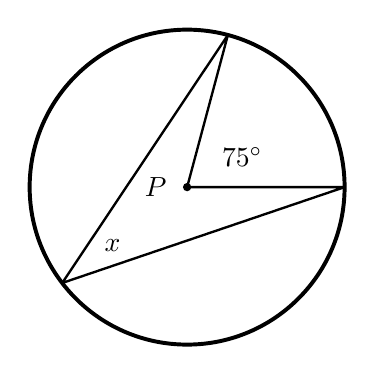
\begin{tikzpicture}[dot/.style={circle, fill=black, inner sep=0pt, outer sep=0pt, minimum size=3pt}, 
dim-label/.style={fill=white, rectangle, inner sep=2pt, outer sep=0pt}, 
nodot/.style={circle, fill=black, inner sep=0pt, outer sep=0pt, minimum size=0pt}, 
%remember picture, overlay
baseline = (current bounding box.west)
]  

% the origin 
\coordinate (p) at (0,0); 
% the circle and the nodot at the origin
\draw[line width=0.5mm] (p) node[circle, fill=black, inner sep=0pt, outer sep=0pt, minimum size=3pt] {} circle [radius=\rad2]; 

\node(p-label) at ($(p)+(180:0.2*\rad2)$) {$P$};

\node(p-angle) at ($(p)+(29:0.4*\rad2)$) {$75\degree$};

\node (a) at (0:\rad2) [nodot] {}; 

\node (b) at (75:\rad2) [nodot] {}; 


\node (c) at (217.5:\rad2) [nodot] {}; 

\node(x-label) at ($(c)+(37:0.4*\rad2)$) {$x$};


\draw[line width=0.3mm] (p)--(a)--(c) --(b) --(p) ; 


\end{tikzpicture} 
%2
\item \hspce 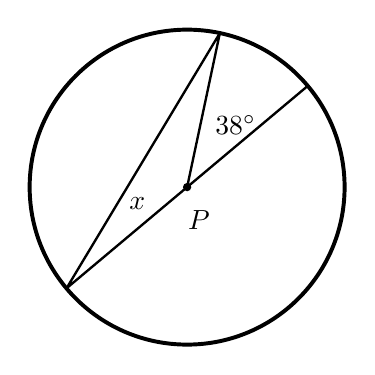
\begin{tikzpicture}[dot/.style={circle, fill=black, inner sep=0pt, outer sep=0pt, minimum size=3pt}, 
dim-label/.style={fill=white, rectangle, inner sep=2pt, outer sep=0pt}, 
nodot/.style={circle, fill=black, inner sep=0pt, outer sep=0pt, minimum size=0pt}, 
%remember picture, overlay
baseline = (current bounding box.west)
]  

\coordinate (p) at (0,0); 

\draw[line width=0.5mm] (p) node[circle, fill=black, inner sep=0pt, outer sep=0pt, minimum size=3pt] {} circle [radius=\rad2]; 

\node(p-label) at ($(p)+(290:0.22*\rad2)$) {$P$};

\node(p-angle) at ($(p)+(52:0.5*\rad2)$) {${38\degree}$};

\node (a) at (40:\rad2) [nodot] {}; 

\node (b) at (78:\rad2) [nodot] {}; 

\node (c) at (220:\rad2) [nodot] {};

\node(x-label) at ($(c)+(50:0.7*\rad2)$) {${x}$};
 
\draw[line width=0.3mm] (a)--(c)--(b)--(p) ; 

\end{tikzpicture} 
%3
\item \hspce 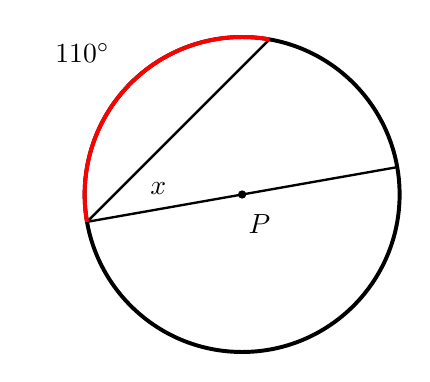
\begin{tikzpicture}[dot/.style={circle, fill=black, inner sep=0pt, outer sep=0pt, minimum size=3pt}, 
dim-label/.style={fill=white, rectangle, inner sep=2pt, outer sep=0pt}, 
nodot/.style={circle, fill=black, inner sep=0pt, outer sep=0pt, minimum size=0pt}, 
%remember picture, overlay
baseline = (current bounding box.west)
]  
\coordinate (p) at (0,0); 

\draw[line width=0.5mm] (p) node[circle, fill=black, inner sep=0pt, outer sep=0pt, minimum size=3pt] {} circle [radius=\rad2]; 

\node(p-label) at ($(p)+(-60:0.22*\rad2)$) {${P}$};

\node(angle) at ($(p)+(140:1.4*\rad2)$) {$ \  \ {110\degree}$};

\node (a) at (10:\rad2) [nodot] {}; 

\node (b) at (80:\rad2) [nodot] {}; 

\node (c) at (190:\rad2) [nodot] {};

\node(x-label) at ($(c)+(25:0.5*\rad2)$) {${x}$};
 
\draw[line width=0.3mm] (a)--(c) --(b); 

\draw[red, line width=0.5mm] (b)  arc (80:190:\rad2);

\end{tikzpicture} 
%4
\item \hspce 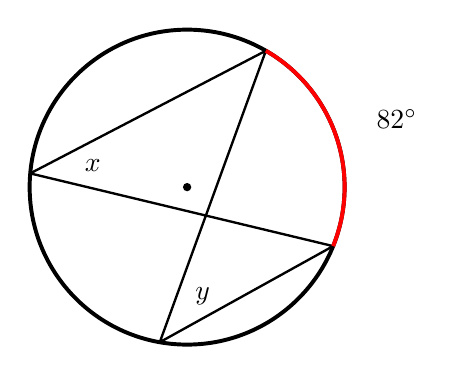
\begin{tikzpicture}[dot/.style={circle, fill=black, inner sep=0pt, outer sep=0pt, minimum size=3pt}, 
dim-label/.style={fill=white, rectangle, inner sep=2pt, outer sep=0pt}, 
nodot/.style={circle, fill=black, inner sep=0pt, outer sep=0pt, minimum size=0pt}, 
%remember picture, overlay
baseline = (current bounding box.west)
]  

\coordinate (p) at (0,0); 

\draw[line width=0.5mm] (p) node[circle, fill=black, inner sep=0pt, outer sep=0pt, minimum size=3pt] {} circle [radius=\rad2];
 
%\node(p-label) at ($(p)+(180:15pt)$) {$ \  \ {P}$};
\node(angle) at ($(p)+(18:1.4*\rad2)$) {${82\degree}$};

\node (a) at (60:\rad2) [nodot] {}; 

\node (b) at (175:\rad2) [nodot] {}; 

\node (c) at (260:\rad2) [nodot] {}; 

\node (d) at (-22:\rad2) [nodot] {};

\node(x-label) at ($(b)+(7:0.4*\rad2)$) {${x}$};

\node(y-label) at ($(c)+(47:0.4*\rad2)$) {${y}$};
 
\draw[line width=0.3mm] (a)--(b) --(d) --(c)--(a); 

\draw[red, line width=0.5mm] (d)  arc (-22:60:\rad2);

\end{tikzpicture} 
%5
\item \hspce 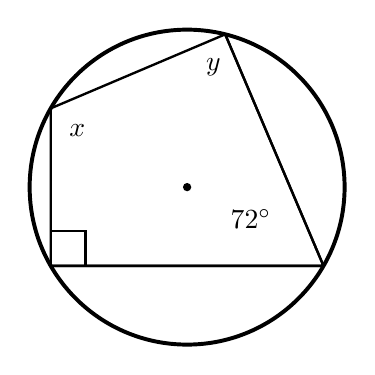
\begin{tikzpicture}[dot/.style={circle, fill=black, inner sep=0pt, outer sep=0pt, minimum size=3pt}, 
dim-label/.style={fill=white, rectangle, inner sep=2pt, outer sep=0pt}, 
nodot/.style={circle, fill=black, inner sep=0pt, outer sep=0pt, minimum size=0pt}, 
%remember picture, overlay
baseline = (current bounding box.west)
]  

\coordinate (p) at (0,0); 

\draw[line width=0.5mm] (p) node[circle, fill=black, inner sep=0pt, outer sep=0pt, minimum size=3pt] {} circle [radius=\rad2]; 

\node (a) at (76:\rad2) [nodot] {};

\node(y-label) at ($(a)+(250:0.22*\rad2)$) {${y}$};
  
\node (b) at (150:\rad2) [nodot] {};

\node(x-label) at ($(b)+(-40:0.22*\rad2)$) {${x}$};
 
\node (c) at (210:\rad2) [nodot] {}; 

\draw[line width=0.3mm] (c) rectangle ++(0.22*\rad2,0.22*\rad2) node[]{};

\node (d) at (-30:\rad2) [nodot] {}; 

\draw [line width=0.3mm](a) -- (d) -- (c) pic [draw,angle radius=0.3*\rad2] {angle = a--d--c}; 

\node(d-angle) at ($(d)+(150:0.6*\rad2)$) {$ \  \ {72\degree}$};

\draw[line width=0.3mm] (a)--(b) --(c) --(d) --(a) ; 

\end{tikzpicture} 
%6
\item \hspce 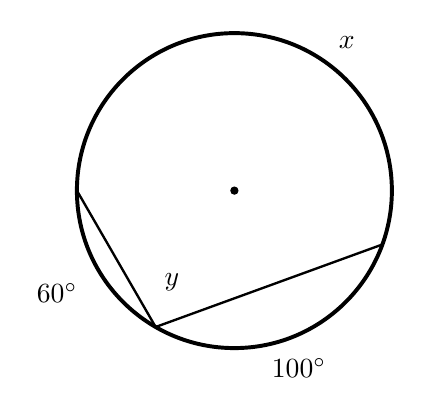
\begin{tikzpicture}[dot/.style={circle, fill=black, inner sep=0pt, outer sep=0pt, minimum size=3pt}, 
dim-label/.style={fill=white, rectangle, inner sep=2pt, outer sep=0pt}, 
nodot/.style={circle, fill=black, inner sep=0pt, outer sep=0pt, minimum size=0pt}, 
%remember picture, overlay
baseline = (current bounding box.west)
]  

\coordinate (p) at (0,0); 

\draw[line width=0.5mm] (p) node[circle, fill=black, inner sep=0pt, outer sep=0pt, minimum size=3pt] {} circle [radius=\rad2]; 

\node (a) at (180:\rad2) [nodot] {}; 

\node (b) at (240:\rad2) [nodot] {};

\node(y-label) at ($(b)+(70:0.3*\rad2)$) {${y}$};
 
\node (c) at (340:\rad2) [nodot] {}; 

\node(ab) at ($(p)+(210:1.3*\rad2)$) {${60\degree}$};

\node(x-label) at ($(c)+(100:1.3*\rad2)$) {$x$};
 
\node(bc) at ($(p)+(290:1.2*\rad2)$) {${100\degree}$};

\draw[line width=0.3mm] (a)--(b) --(c); 

\end{tikzpicture} 
%7
\item \hspce 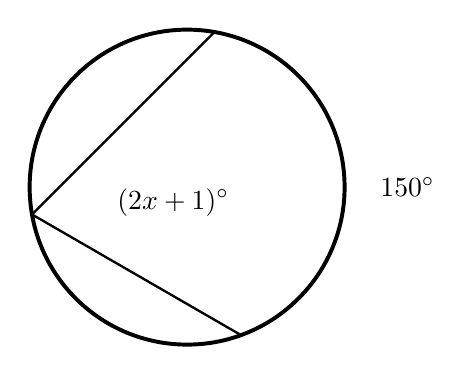
\begin{tikzpicture}[dot/.style={circle, fill=black, inner sep=0pt, outer sep=0pt, minimum size=3pt}, 
dim-label/.style={fill=white, rectangle, inner sep=2pt, outer sep=0pt}, 
nodot/.style={circle, fill=black, inner sep=0pt, outer sep=0pt, minimum size=0pt}, 
%remember picture, overlay
baseline = (current bounding box.west)
]  

\coordinate (p) at (0,0); 

\draw[line width=0.5mm] (p) node[circle, fill=black, inner sep=0pt, outer sep=0pt, minimum size=0pt] {} circle [radius=\rad2]; 

\node (a) at (80:\rad2) [nodot] {}; 

\node (b) at (190:\rad2) [nodot] {}; 

\node (c) at (-70:\rad2) [nodot] {}; 

\draw[line width=0.3mm] (a)--(b)--(c); 

\node(measure) at ($(b)+(5:0.9*\rad2)$) {${(2x+1)\degree}$};
 
\node(angle) at ($(p)+(0:1.4*\rad2)$) {${150\degree}$};
 
\end{tikzpicture} 
%8
\item \hspce 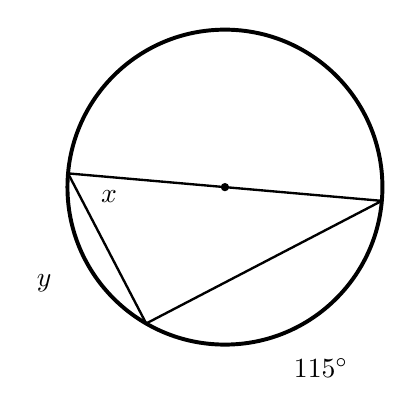
\begin{tikzpicture}[dot/.style={circle, fill=black, inner sep=0pt, outer sep=0pt, minimum size=3pt}, 
dim-label/.style={fill=white, rectangle, inner sep=2pt, outer sep=0pt}, 
nodot/.style={circle, fill=black, inner sep=0pt, outer sep=0pt, minimum size=0pt}, 
%remember picture, overlay
baseline = (current bounding box.west)
]  

\coordinate (p) at (0,0); 

\draw[line width=0.5mm] (p) node[circle, fill=black, inner sep=0pt, outer sep=0pt, minimum size=3pt] {} circle [radius=\rad2]; 

\node (a) at (-5:\rad2) [nodot] {}; 

\node (b) at (175:\rad2) [nodot] {}; 

\node (c) at (240:\rad2) [nodot] {}; 

\draw[line width=0.3mm] (a)--(b)--(c)--(a) ; 
 
\node(y-label) at ($(p)+(208:1.3*\rad2)$) {${y}$};
 
\node(x-label) at ($(b)+(-30:0.3*\rad2)$) {${x}$};
 
\node(115) at ($(p)+(298:1.3*\rad2)$) {${115\degree}$};
 
\end{tikzpicture} 
\end{multicols}
\end{enumerate}}     
\end{minipage}}
\end{center} 

B. $\Delta$GOA is inscribed in $\odot L$. If $m\angle{OGA}=75\degree$ and $m\arc{AG}=160\degree$, find: 
\begin{center}
\scalebox{0.5}{
\noindent\begin{minipage}{0.3\textwidth}
 
{\begin{enumerate}[label = \arabic*. ]
\item $m\arc{OA}$ 
\item $m\arc{OG}$
\item $m\angle{GOA}$ \hspace*{3cm}\begin{tikzpicture}[dot/.style={circle, fill=black, inner sep=0pt, outer sep=0pt, minimum size=3pt}, 
dim-label/.style={fill=white, rectangle, inner sep=2pt, outer sep=0pt}, 
nodot/.style={circle, fill=black, inner sep=0pt, outer sep=0pt, minimum size=0pt}, 
remember picture, overlay
]  

\def\rad4{1.3cm}

\coordinate (l) at (0,0); 

\node(l-label) at ($(l)+(30:0.22*\rad4)$) {$L$};

\draw[line width=0.5mm] (l) node[circle, fill=black, inner sep=0pt, outer sep=0pt, minimum size=3pt] {} circle [radius=\rad4]; 

\node (a) at (15:\rad4) [nodot] {}; 

\node(a-label) at ($(a)+(15:0.22*\rad4)$) {$A$};
  
\node (o) at (165:\rad4) [nodot] {}; 

\node(o-label) at ($(o)+(165:0.22*\rad4)$) {$O$};
  
\node (g) at (215:\rad4) [nodot] {};

\node(g-label) at ($(g)+(215:0.22*\rad4)$) {$G$};
   
\node(75) at ($(g)+(53:0.4*\rad4)$) {$75\degree$};

\draw[line width=0.3mm] (a)--(o)--(g)--(a) ; 
 
\node(160) at ($(l)+(-45:1.3*\rad4)$) {$160\degree$};

\draw[red, line width=0.5mm] (a)  arc (15:-145:\rad4);

\end{tikzpicture} 
\item $m\angle{GAO}$  
\end{enumerate}}
\end{minipage}}
\end{center} }



\def \EvaluationDayA {
\input{/storage/emulated/0/Documents/documents/latex/1920/Grade-10/2nd/inscribed-angles-and-intercepted-arcs/qz-inscribed-angles-and-intercepted-arcs-input} 
}

\def \RemediationDayA {}

\def \LessonDayB {Radii and Chords}

\def \LearningCompetenciesDayB {}

\def \ObjectivesDayB {
\item %cogverbstart
Recall
%cogverbend
the radii and chords; 
\item %psyverbstart
Compute
%psyverbend
the radii and chords to determine whether a binomial is a factor of a given polynomial; and, 
\item %affverbstart
Demonstrate
%affverbend
%valsstart
enjoyment and willingness
%valsend
in solving problems.
}

\def \PurposeDayB {The purpose of this lesson is to enable the students to solve real life problems involving the radii and chords.}  

\def \ApplicationDayB { Let the students answer the following questions: 
\begin{enumerate}[label = \arabic*. ]
%1
\item In what real life situations or problems can we observe some examples of radii and chords? 
%2
\item How can you apply your knowledge of radii and chords in solving these real life problems? 

\end{enumerate}   
}

\def \GeneralizationDayB {Let the students answer the following questions: 
\begin{enumerate}[label = \arabic*. ]
%1
\item In your own words, what is the radii and chords? 
%2
\item How do we solve problems involving radii and chords? 

\end{enumerate}   
}

\def \TeachersGuideDayB {pp. 131--134}

\def \LMPagesDayB {pp. 120--123}

\def \TextbookPagesDayB {pp. 128--132}

\def \AdditionalMaterialsDayB {}

\def \OtherResourcesDayB {Flashcards}

\def \ReviewDayB {\begin{center}
\textbf{Radii and Chords}
\end{center}

\vspace*{1ex}

\begin{center}
\scalebox{0.5}{
\noindent\begin{minipage}{0.3\textwidth}

{
\textbf{Perpendicular to a Chord Theorem:} The perpendicular from the center of the circle to any chord bisects the chord. 

\vspce 

\textbf{Center to Chord Midpoint Theorem:} The line joining the center of the circle to the midpoint of any chord which is not a diameter is perpendicular to the chord. 

\vspce 

\textbf{Perpendicular Bisector Chord to Center Theorem:}  The perpendicular bisector of a chord of a circle passes through the center of the circle. 

\vspce 

\textbf{Perpendicular Bisector Chord to Central Angle Theorem:} The perpendicular bisector of a chord of a circle bisects the central angle subtended by the chord. 

\vspce 

\textbf{Central Angle Bisector Theorem:} The bisector of a central angle subtended by the chord is the perpendicular bisector of the chord. 

\vspce 

\textbf{Distance--Chord Theorem:} In the same circle or in congruent circles, chords are congruent if and only if their distances from the center(s) of the circle(s) are equal. 


\vspce 

\textbf{Chord -- Arc Congruence Theorem:} In a circle or in congruent circles, two minor arcs are congruent if and only if their corresponding chords are congruent. 
}
\end{minipage}}
\end{center} 

 


 




}



\def \ExamplesDayB {}

\def \PracticeOneDayB {\def\currentdir{/storage/emulated/0/Documents/documents/latex/1920/Grade-10/2nd/radii-and-chords}

\textbf{Practice Exercises}

\vspace*{-2ex}

\begin{center}
\scalebox{0.5}{
\noindent\begin{minipage}{0.3\textwidth}
{
A. In $\odot{I}$, $\overline{PH}$ and $\overline{CE}$ are diameters with $\overline{PH}\perp\overline{AE}$ and $\overline{PH}\perp\overline{CU}$. 

\begin{enumerate}[label = \arabic*. ]
\item Name the midpoint of $\overline{PH}$. 
\item Name the midpoint of $\overline{CE}$.
\item Name the midpoint of $\overline{AE}$. %\hspace*{6cm}\vspace*{0ex}
\begin{tikzpicture}[dot/.style={circle, fill=black, inner sep=0pt, outer sep=0pt, minimum size=4pt},
nodot/.style={circle, fill=black, inner sep=0pt, outer sep=0pt, minimum size=0pt},
 remember picture, overlay
]

\def\radfig1{1.5cm}

\node(i)[dot] at (0,0) {};

\draw[name path=circ, line width=0.4mm] (i) circle (\radfig1);

\node(i-label) at ($(i)+(120:0.18*\radfig1)$) {$\  I$};

\coordinate (p) at ($(i) +(180:\radfig1)$);

\node(p-label) at ($(p)+(180:0.22*\radfig1)$) {$\  P$};

\coordinate (h) at ($(i) +(0:\radfig1)$);

\node(h-label) at ($(h)+(0:0.1*\radfig1)$) {$\  H$};

\node[nodot] (w) at ($(p)!0.5!(i)$){};

\node(w-label) at ($(w)+(145:0.25*\radfig1)$) {$\  W$};

\node[nodot] (n) at ($(i)!0.5!(h)$){};

\node(n-label) at ($(n)+(60:0.15*\radfig1)$) {$\  N$};

\path[name path=line1.guess, line width=0.5mm] (n) -- ($(n)!3!-90:(i)$);

\fill[black, name intersections={of=line1.guess and circ, name=point}];

\node[nodot] (c) at (point-1){};

\node(c-label) at ($(c)+(90:0.22*\radfig1)$) {$\  C$};

\path[name path=line2.guess, line width=0.5mm] (n) -- ($(n)!3!90:(i)$);

\fill[black, name intersections={of=line2.guess and circ, name=point}];

\node[nodot] (u) at (point-1){};

\node(u-label) at ($(u)+(-90:0.22*\radfig1)$) {$\  U$};

\path[name path=line3.guess, line width=0.5mm] (w) -- ($(w)!3!90:(i)$);

\fill[black, name intersections={of=line3.guess and circ, name=point}];

\node[nodot] (a) at (point-1){};

\node(a-label) at ($(a)+(110:0.22*\radfig1)$) {$\  A$};

\path[name path=line4.guess, line width=0.5mm] (w) -- ($(w)!3!-90:(i)$);

\fill[black, name intersections={of=line4.guess and circ, name=point}];

\node[nodot] (e) at (point-1){};

\node(e-label) at ($(e)+(-120:0.22*\radfig1)$) {$\  E$};

\draw[line width=0.5mm] (p) -- (h);

\draw[line width=0.5mm] (a) -- (e);

\draw[line width=0.5mm] (e) -- (c);

\draw[line width=0.5mm] (c) -- (u);


\end{tikzpicture}
\vspace*{-1.5ex}
\item Name the midpoint of $\overline{CU}$.
\item If $\overline{IW}\cong\overline{IN}$, name a chord  congruent \newline
 to $\overline{AE}$ and an arc  congruent to $\arc{CHU}$. 
\item Name two arcs congruent to $\arc{AP}$. 
\end{enumerate}  
\vspace*{-2.5cm}\hspace*{8.5cm}
\begin{tikzpicture}[dot/.style={circle, fill=black, inner sep=0pt, outer sep=0pt, minimum size=4pt},
nodot/.style={circle, fill=black, inner sep=0pt, outer sep=0pt, minimum size=0pt},
 remember picture, overlay
]

\def\radfig1{1.5cm}

\node(i)[dot] at (0,0) {};

\draw[name path=circ, line width=0.4mm] (i) circle (\radfig1);

\node(i-label) at ($(i)+(120:0.18*\radfig1)$) {$\  I$};

\coordinate (p) at ($(i) +(180:\radfig1)$);

\node(p-label) at ($(p)+(180:0.22*\radfig1)$) {$\  P$};

\coordinate (h) at ($(i) +(0:\radfig1)$);

\node(h-label) at ($(h)+(0:0.1*\radfig1)$) {$\  H$};

\node[nodot] (w) at ($(p)!0.5!(i)$){};

\node(w-label) at ($(w)+(145:0.25*\radfig1)$) {$\  W$};

\node[nodot] (n) at ($(i)!0.5!(h)$){};

\node(n-label) at ($(n)+(60:0.15*\radfig1)$) {$\  N$};

\path[name path=line1.guess, line width=0.5mm] (n) -- ($(n)!3!-90:(i)$);

\fill[black, name intersections={of=line1.guess and circ, name=point}];

\node[nodot] (c) at (point-1){};

\node(c-label) at ($(c)+(90:0.22*\radfig1)$) {$\  C$};

\path[name path=line2.guess, line width=0.5mm] (n) -- ($(n)!3!90:(i)$);

\fill[black, name intersections={of=line2.guess and circ, name=point}];

\node[nodot] (u) at (point-1){};

\node(u-label) at ($(u)+(-90:0.22*\radfig1)$) {$\  U$};

\path[name path=line3.guess, line width=0.5mm] (w) -- ($(w)!3!90:(i)$);

\fill[black, name intersections={of=line3.guess and circ, name=point}];

\node[nodot] (a) at (point-1){};

\node(a-label) at ($(a)+(110:0.22*\radfig1)$) {$\  A$};

\path[name path=line4.guess, line width=0.5mm] (w) -- ($(w)!3!-90:(i)$);

\fill[black, name intersections={of=line4.guess and circ, name=point}];

\node[nodot] (e) at (point-1){};

\node(e-label) at ($(e)+(-120:0.22*\radfig1)$) {$\  E$};

\draw[line width=0.5mm] (p) -- (h);

\draw[line width=0.5mm] (a) -- (e);

\draw[line width=0.5mm] (e) -- (c);

\draw[line width=0.5mm] (c) -- (u);


\end{tikzpicture}
\vspace*{2.5cm}
}
\end{minipage}}
\end{center} 
}

\def \PracticeTwoDayB {\def\currentdir{/storage/emulated/0/Documents/documents/latex/1920/Grade-10/2nd/radii-and-chords}

\begin{center}
\vspace*{-2ex}
\scalebox{0.5}{
\noindent\begin{minipage}{0.3\textwidth}
{
B. In $\odot{T}$, $\overline{AT}$ is a radius and $\overline{AL}$ is a chord. 
\begin{enumerate}[label = \arabic*. ]

\item If $\overline{TK}\perp\overline{AL}$, then $\overline{TK}\blank\overline{AL}$. 
\item If $\overrightarrow{TK}$ bisects $\angle{ATL}$, then  $\overrightarrow{TK}\blank\overline{AL}$. 
\item If $\overline{TK}$ is a perpendicular  bisector \newline of $\overline{AL}$, then $\overrightarrow{TK}\blank\angle{ATL}$. 
\item The altitude $\overrightarrow{TK}$ to the base of \newline $\Delta{ATL}$ is also a \blank. 
\end{enumerate}  
\vspace*{-2.8cm}\hspace*{8.5cm}
\begin{tikzpicture}[dot/.style={circle, fill=black, inner sep=0pt, outer sep=0pt, minimum size=4pt},
nodot/.style={circle, fill=black, inner sep=0pt, outer sep=0pt, minimum size=0pt},
 remember picture, overlay
]

\def\radfig2{1.5cm}

\node(t)[dot] at (0,0) {};

\draw[name path=circ, line width=0.5mm] (t) circle (\radfig2);

\node(t-label) at ($(t)+(180:0.22*\radfig2)$) {$\  T$};

\coordinate (b) at ($(t) +(0:\radfig2)$);

\node[nodot] (k) at ($(t)!0.5!(b)$){};

\node(k-label) at ($(k)+(45:0.22*\radfig2)$) {$\  K$};

\path[name path=line.guess, line width=0.5mm] (k) -- ($(k)!3!-90:(t)$);

\fill[black, name intersections={of=line.guess and circ, name=point}];

\node[nodot] (a) at (point-1){};

\node(a-label) at ($(a)+(70:0.22*\radfig2)$) {$\  A$};

\path[name path=line2.guess, line width=0.5mm] (k) -- ($(k)!3!90:(t)$);

\fill[black, name intersections={of=line2.guess and circ, name=point}];

\node[nodot] (l) at (point-1){};

\node(l-label) at ($(l)+(-90:0.22*\radfig2)$) {$\  L$};

\draw[line width=0.5mm] (a) -- (t);

\draw[line width=0.5mm, ->, >={Latex[round]}] (t) -- ($(t)!1.3!(b)$);

\draw[line width=0.5mm] (a) -- (l) -- (t) ;

%\node(figure2) at ($(t)+(-90:1.3*\radfig2)$) {\LARGE Figure for Nos. 7--10};

\end{tikzpicture}

\vspace*{2.8cm}
}
\end{minipage}}
\end{center} 
}

\def \MasteryDayB {\def\radfig3a{1.5cm}
\def\currentdir{/storage/emulated/0/Documents/documents/latex/1920/Grade-10/2nd/radii-and-chords}

\textbf{Problem Set}

\vspce

Find the value of $x$ in each figure. 

\begin{center}
\scalebox{0.5}{
\noindent\begin{minipage}{0.3\textwidth}
{\begin{tabularx}{\textwidth}{XX}

1. \begin{tikzpicture}[dot/.style={circle, fill=black, inner sep=0pt, outer sep=0pt, minimum size=3pt}, 
nodot/.style={circle, fill=black, inner sep=0pt, outer sep=0pt, minimum size=0pt}, 
%remember picture,% overlay
baseline = (current bounding box.west)
]  

\node(i)[dot] at (0,0) {};

\draw[name path=circ, line width=0.5mm] (i) circle (\radfig3a);

\coordinate (f) at ($(i) +(\radfig3a, 0)$);

\coordinate (g) at ($(i) -(\radfig3a, 0)$);

\coordinate (int1) at ($(i)! 0.66!(f)$);

\coordinate (int2) at ($(i)! 0.66!(g)$);

\coordinate (tick1) at ($(i)! 0.33!(f)$);

\coordinate (tick2) at ($(i)! 0.33!(g)$);

\draw[line width=0.3mm] ($(tick1)+(0,0.1*\radfig3a)$) -- ($(tick1)-(0,0.1*\radfig3a)$);

\draw[line width=0.3mm] ($(tick2)+(0,0.1*\radfig3a)$) -- ($(tick2)-(0,0.1*\radfig3a)$); 

\node(x.label) at ($(int1)+(30:0.13*\radfig3a)$) {$x$};

\node(12-label) at ($(int2)+(150:0.22*\radfig3a)$) {$12$};

\path[name path=line1.guess, line width=0.5mm] (int1) -- ($(int1)!3!90:(i)$);

\fill[black, name intersections={of=line1.guess and circ, name=point}];

\node[nodot] (d) at (point-1){};

\node(d-label) at ($(d)+(-60:0.22*\radfig3a)$) {$\  D$};

\path[name path=line2.guess, line width=0.5mm] (int1) -- ($(int1)!3!-90:(i)$);

\fill[black, name intersections={of=line2.guess and circ, name=point}];

\node[nodot] (c) at (point-1){};

\node(c-label) at ($(c)+(60:0.22*\radfig3a)$) {$\  C$};

\path[name path=line3.guess, line width=0.5mm] (int2) -- ($(int2)!3!90:(i)$);

\fill[black, name intersections={of=line3.guess and circ, name=point}];

\node[nodot] (a) at (point-1){};

\node(a-label) at ($(a)+(120:0.22*\radfig3a)$) {$\  A$};

\path[name path=line4.guess, line width=0.5mm] (int2) -- ($(int2)!3!-90:(i)$);

\fill[black, name intersections={of=line4.guess and circ, name=point}];

\node[nodot] (b) at (point-1){};

\node(b-label) at ($(b)+(240:0.22*\radfig3a)$) {$\  B$};

\draw[line width=0.5mm] (int2) -- (int1) ;

\draw[line width=0.5mm] (c) -- (d) ;

\draw[line width=0.5mm] (a) -- (b) ;

\begin{scope} [rotate=180]
\draw[line width=0.3mm] (int1) rectangle ++(0.22*\radfig3a,0.22*\radfig3a) node[transform shape]{};
\end{scope}

\begin{scope} [rotate=0]
\draw[line width=0.3mm] (int2) rectangle ++(0.22*\radfig3a,0.22*\radfig3a) node[transform shape]{};
\end{scope}

\end{tikzpicture}

  & 5. \begin{tikzpicture}[dot/.style={circle, fill=black, inner sep=0pt, outer sep=0pt, minimum size=3pt}, 
%dim-label/.style={fill=white, rectangle, inner sep=2pt, outer sep=0pt}, 
nodot/.style={circle, fill=black, inner sep=0pt, outer sep=0pt, minimum size=0pt}, 
%remember picture, overlay, 
baseline = (current bounding box.west)
] 

\node(i)[dot] at (0,0) {};

\draw[name path=circ, line width=0.5mm] (i) circle (\radfig3a);

\coordinate (a) at ($(i) + (100:\radfig3a)$);

\coordinate (b) at ($(i) + (220:\radfig3a)$);

\coordinate (c) at ($(i) + (340:\radfig3a)$);

\coordinate (int) at ($(a)! 0.5!(c)$);

\node(a.label) at ($(a)+(100:0.22*\radfig3a)$) {$  A$};

\node(b.label) at ($(b)+(220:0.22*\radfig3a)$) {$  B$};

\node(c.label) at ($(c)+(340:0.22*\radfig3a)$) {$  C$};

\node(x.label) at ($(int)+(40:0.13*\radfig3a)$) {$  x$};

\pic [draw, line width=0.3mm, angle radius=0.25*\radfig3a] {angle=b--a--c};

\pic [draw, line width=0.3mm, angle radius=0.25*\radfig3a] {angle=a--c--b};

\pic [draw, line width=0.3mm, angle radius=0.25*\radfig3a] {angle=c--b--a};
 
\draw[line width=0.3mm] ($(a)! 0.15*\radfig3a! (i) $) -- ($(a)! 0.35*\radfig3a! (i) $) ;

\draw[line width=0.3mm] ($(b)! 0.15*\radfig3a! (i) $) -- ($(b)! 0.35*\radfig3a! (i) $) ;

\draw[line width=0.3mm] ($(c)! 0.15*\radfig3a! (i) $) -- ($(c)! 0.35*\radfig3a! (i) $) ;

\draw[line width=0.5mm] (a) -- (b) node[midway, xshift=-0.22*\radfig3a] (17.label) {$17$};;

\draw[line width=0.5mm] (c) -- (b) ;

\draw[line width=0.5mm] (a) -- (c) ;

\draw[line width=0.3mm, densely dotted] (b) -- (int) ;

\begin{scope} [rotate=-140]
\draw[line width=0.3mm] (int) rectangle ++(0.22*\radfig3a,0.22*\radfig3a) node[transform shape]{};
\end{scope}

\end{tikzpicture}

\\
2. \begin{tikzpicture}[dot/.style={circle, fill=black, inner sep=0pt, outer sep=0pt, minimum size=3pt}, 
nodot/.style={circle, fill=black, inner sep=0pt, outer sep=0pt, minimum size=0pt}, 
%remember picture, overlay, 
baseline = (current bounding box.west)
]  

\node(i)[dot] at (0,0) {};

\draw[name path=circ, line width=0.5mm] (i) circle (\radfig3a);

\coordinate (b) at ($(i) +(120:\radfig3a)$);

\node(b-label) at ($(b)+(120:0.22*\radfig3a)$) {$\  B$};

\coordinate (c) at ($(i) +(70:\radfig3a)$);

\node(c-label) at ($(c)+(70:0.22*\radfig3a)$) {$\  C$};

\coordinate (e) at ($(i) +(250:\radfig3a)$);

\node(e-label) at ($(e)+(250:0.22*\radfig3a)$) {$E$};

\coordinate (int1) at ($(i)! 0.66!(e)$);

\path[name path=line.guess, line width=0.5mm] ($(int1)!2!-90:(i)$) -- ($(int1)!2!90:(i)$);

\fill[black, name intersections={of=line.guess and circ, name=point}];

\node[nodot] (a) at (point-1){};

\node[nodot] (d) at (point-2){};

\node(a-label) at ($(a) +(160:0.22*\radfig3a)$) {$\  A$};

\node(d-label) at ($(d) +(-20:0.22*\radfig3a)$) {$\  D$};

\node(50-label) at ($(int1) +(200:0.8*\radfig3a)$) {$\  50\degree$};

\node(x.label) at ($(int1) +(-60:0.6*\radfig3a)$) {$x$};

\draw[line width=0.3mm] (a) -- (d) ;

\draw[line width=0.3mm] (c) -- (e) ;

\draw[line width=0.3mm] (i) -- (b) ;

\begin{scope} [rotate=160]
\draw[line width=0.3mm] (int1) rectangle ++(0.22*\radfig3a,0.22*\radfig3a) node[transform shape]{};
\end{scope}

\end{tikzpicture}

  & 6. \begin{tikzpicture}[dot/.style={circle, fill=black, inner sep=0pt, outer sep=0pt, minimum size=3pt}, 
%dim-label/.style={fill=white, rectangle, inner sep=2pt, outer sep=0pt}, 
nodot/.style={circle, fill=black, inner sep=0pt, outer sep=0pt, minimum size=0pt}, 
%remember picture, overlay, 
baseline = (current bounding box.west)
] 

\node(c)[dot] at (0,0) {};

\draw[name path=circ, line width=0.5mm] (c) circle (\radfig3a);

\node(c-label) at ($(c)+(225:0.22*\radfig3a)$) {$\  C$};

\coordinate (a) at ($(i) + (0, \radfig3a)$);

\coordinate (b) at ($(i) +(\radfig3a, 0)$);

\coordinate (int) at ($(a)! 0.5!(b)$);

\node(a.label) at ($(a)+(90:0.22*\radfig3a)$) {$\  A$};

\node(b.label) at ($(b)+(0:0.19*\radfig3a)$) {$B$};

\draw[line width=0.3mm] (a) -- (c) node [midway, xshift=-0.12*\radfig3a] (6.label) {$6$} -- (b) ;

\draw[line width=0.3mm] (a) -- (b) node [midway, xshift=0.11*\radfig3a, yshift=0.09*\radfig3a] (x.label) {$x$};

\draw[line width=0.3mm] (c) -- (int) ;

\begin{scope} [rotate=135]
\draw[line width=0.3mm] (int) rectangle ++(0.22*\radfig3a,0.22*\radfig3a) node[transform shape]{};
\end{scope}

\begin{scope} [rotate=0]
\draw[line width=0.3mm] (c) rectangle ++(0.22*\radfig3a,0.22*\radfig3a) node[transform shape]{};
\end{scope}

\end{tikzpicture}

\\
3. \begin{tikzpicture}[dot/.style={circle, fill=black, inner sep=0pt, outer sep=0pt, minimum size=3pt}, 
%dim-label/.style={fill=white, rectangle, inner sep=2pt, outer sep=0pt}, 
nodot/.style={circle, fill=black, inner sep=0pt, outer sep=0pt, minimum size=0pt}, 
%remember picture, overlay, 
baseline = (current bounding box.west)
] 

\node(o)[dot] at (0,0) {};

\draw[name path=circ, line width=0.5mm] (o) circle (\radfig3a);

\node(o-label) at ($(o)+(170:0.22*\radfig3a)$) {$  O$};

\coordinate (c) at ($(o) -(0,\radfig3a)$);

\node(c.label) at ($(c)+(-90:0.22*\radfig3a)$) {$  C$};

\coordinate (d) at ($(o) +(0,\radfig3a)$);

\node(d.label) at ($(d)+(90:0.22*\radfig3a)$) {$  D$};

\coordinate (e) at ($(o) +(50:\radfig3a)$);

\node(e.label) at ($(e)+(50:0.22*\radfig3a)$) {$  E$};

\coordinate (int1) at ($(o)! 0.55!(c)$);

\path[name path=line.guess, line width=0.5mm] ($(int1)!2!-90:(i)$) -- ($(int1)!2!90:(i)$);

\fill[black, name intersections={of=line.guess and circ, name=point}];

\node[nodot] (a) at (point-1){};

\node(a-label) at ($(a)+(180:0.22*\radfig3a)$) {$  A$};

\node[nodot] (b) at (point-2){};

\node(b.label) at ($(b)+(0:0.22*\radfig3a)$) {$  B$};

\draw[line width=0.3mm] (c) -- (d) ;

\draw[line width=0.3mm] (a) -- (b) ;

\draw[line width=0.3mm] (o) -- (e) node[midway, xshift=0.15*\radfig3a, yshift=-0.2*\radfig3a] (8.4.label) {$  8.4$};

\begin{scope} [rotate=0]
\draw[line width=0.3mm] (int1) rectangle ++(0.22*\radfig3a,0.22*\radfig3a) node[transform shape]{};
\end{scope}

\coordinate (tick1) at ($(int1)!0.5!(a)$);

\coordinate (tick2) at ($(int1)!0.5!(b)$);

\draw[line width=0.3mm] ($(tick1)+(0,0.07*\radfig3a)$) -- ($(tick1)-(0,0.07*\radfig3a)$);

\draw[line width=0.3mm] ($(tick2)+(0,0.07*\radfig3a)$) -- ($(tick2)-(0,0.07*\radfig3a)$);

\draw [decorate, decoration={brace, amplitude=0.5*\radfig3a, mirror}, line width=0.3mm% xshift=-4pt, yshift=0pt
]
(d) -- (c) node [black, midway, xshift=-0.7*\radfig3a] 
{$x$};

\end{tikzpicture}
 & 7. \begin{tikzpicture}[dot/.style={circle, fill=black, inner sep=0pt, outer sep=0pt, minimum size=3pt}, 
nodot/.style={circle, fill=black, inner sep=0pt, outer sep=0pt, minimum size=0pt}, 
baseline = (current bounding box.west)
]  

\node(e)[dot] at (0,0) {};

\draw[name path=circ, line width=0.5mm] (e) circle (\radfig3a);

\node(e.label) at ($(e)+(-20:0.22*\radfig3a)$) {$  E$};

\coordinate (r) at ($(e) +(50:\radfig3a)$);

\coordinate (b) at ($(e) +(180:\radfig3a)$);

\coordinate (c) at ($(e) +(280:\radfig3a)$);

\coordinate (int) at ($(e)! 0.7!(b)$);

\path[name path=line.guess, line width=0.3mm] ($(int)!2!-90:(e)$) -- ($(int)!2!90:(e)$);

\fill[black, name intersections={of=line.guess and circ, name=point}];

\node[nodot] (a) at (point-1){};

\node[nodot] (d) at (point-2){};

\node(d-label) at ($(d)+(250:0.22*\radfig3a)$) {$  D$};

\node(a-label) at ($(a)+(120:0.22*\radfig3a)$) {$  A$};

\draw[line width=0.3mm] (r) -- (e) node [midway, yshift=0.14*\radfig3a, xshift=-0.22*\radfig3a] (25.label) {$25$} -- (c) ;

\draw[line width=0.3mm] (a) -- (d) node [midway, xshift=-0.15*\radfig3a] (14.label) {$14$};;

\draw[line width=0.3mm] (int) -- (e) node [midway, yshift=-0.12*\radfig3a] (x.label) {$x$};

\begin{scope} [rotate=0]
\draw[line width=0.3mm] (int) rectangle ++(0.22*\radfig3a,0.22*\radfig3a) node[transform shape]{};
\end{scope}

\end{tikzpicture}

\\
4. \begin{tikzpicture}[dot/.style={circle, fill=black, inner sep=0pt, outer sep=0pt, minimum size=3pt}, 
nodot/.style={circle, fill=black, inner sep=0pt, outer sep=0pt, minimum size=0pt}, 
baseline = (current bounding box.west)
]  

\node(o)[dot] at (0,0) {};

\draw[name path=circ, line width=0.5mm] (o) circle (\radfig3a);

\node(o-label) at ($(o)+(250:0.22*\radfig3a)$) {$\  O$};

\coordinate (y) at ($(o) +(\radfig3a, 0)$);

\node(y.label) at ($(y)+(0:0.22*\radfig3a)$) {$\  Y$};

\coordinate (a) at ($(o) + (0, \radfig3a)$);

\coordinate (int) at ($(o)! 0.6!(a)$);

\path[name path=line.guess, line width=0.3mm] ($(int)!2.3!-90:(o)$) -- ($(int)!2!90:(o)$);

\fill[black, name intersections={of=line.guess and circ, name=point}];

\node[nodot] (l) at (point-1){};

\node(l.label) at ($(l)+(0:0.22*\radfig3a)$) {$\  L$};

\draw[line width=0.3mm] (o) -- (y) node [midway, yshift=-0.19*\radfig3a] (25)
{$\  25$};

\draw[line width=0.3mm] (o) -- (int) node [midway, xshift=-0.2*\radfig3a, yshift=-2pt] (7)
{$\  7$};;

\draw[line width=0.3mm] (point-2) -- (l) node [midway, yshift=0.15*\radfig3a] (x)
{$\  x$};;

\begin{scope} [rotate=-90]
\draw[line width=0.3mm] (int) rectangle ++(0.22*\radfig3a,0.22*\radfig3a) node[transform shape]{};
\end{scope}

\end{tikzpicture}

  & 8. \begin{tikzpicture}[dot/.style={circle, fill=black, inner sep=0pt, outer sep=0pt, minimum size=3pt}, 
nodot/.style={circle, fill=black, inner sep=0pt, outer sep=0pt, minimum size=0pt}, 
baseline = (current bounding box.west)
] 

\node(i)[dot] at (0,0) {};

\draw[name path=circ, line width=0.5mm] (i) circle (\radfig3a);

\coordinate (r) at ($(i) +(-90:\radfig3a)$);

\coordinate (b) at ($(i) +(-30:\radfig3a)$);

\coordinate (c) at ($(i) +(210:\radfig3a)$);

\coordinate (int1) at ($(i)! 0.5!(b)$);

\coordinate (int2) at ($(i)! 0.5!(c)$);

\coordinate (tick1) at ($(i)! 0.5!(int1)$);

\coordinate (tick2) at ($(i)! 0.5!(int2)$);

\node(r.label) at ($(r)+(-90:0.22*\radfig3a)$) {$  R$};

\path[name path=line.guess, line width=0.3mm] ($(int1)!3!-90:(i)$) -- ($(int1)!3!90:(i)$);

\fill[black, name intersections={of=line.guess and circ, name=point}];

\node[nodot] (a) at (point-1){};

\node(a-label) at ($(a)+(60:0.22*\radfig3a)$) {$  A$};

\path[name path=line2.guess, line width=0.3mm] ($(int2)!2.5!-90:(i)$) -- ($(int2)!2.5!90:(i)$);

\fill[black, name intersections={of=line2.guess and circ, name=point}];

\node[nodot] (p) at (point-1){};

\node(p.label) at ($(p)+(150:0.22*\radfig3a)$) {$  P$};

\node(50.label) at ($(int1)+(-10:0.22*\radfig3a)$) {$  50$};

\node(t.label) at ($(int1)+(100:0.22*\radfig3a)$) {$  T$};

\node(y.label) at ($(int2)+(70:0.22*\radfig3a)$) {$  Y$};

\draw[line width=0.3mm] (int1) -- (i) -- (int2) ;

\draw[line width=0.3mm] (a) -- (r) ;

\draw[line width=0.3mm] (p) --  (int2) -- (r) node [midway, xshift=0.12*\radfig3a, yshift=2pt] (x.label) {$x $}; 

\begin{scope} [rotate=150]
\draw[line width=0.3mm] (int1) rectangle ++(0.2*\radfig3a,0.2*\radfig3a) node[transform shape]{};
\end{scope}

\begin{scope} [rotate=-60]
\draw[line width=0.3mm] (int2) rectangle ++(0.2*\radfig3a,0.2*\radfig3a) node[transform shape]{};
\end{scope}

%\begin{scope} [rotate=60]
\tikzset{mytick/.pic={\draw[line width=0.3mm] ($(0,0)+(0,0.1*\radfig3a)$) -- ($(0,0)-(0,0.1*\radfig3a)$) ; }}
%\end{scope}

\pic[rotate=-30] at (tick1) [pic type = mytick];

\pic[rotate=30] at (tick2) [pic type = mytick];

\end{tikzpicture}

\\

\end{tabularx}}
\end{minipage}}
\end{center} 


}



\def \EvaluationDayB {
\input{/storage/emulated/0/Documents/documents/latex/1920/Grade-10/2nd/radii-and-chords/qz-radii-and-chords-input} 
}

\def \RemediationDayB {}

\def \LessonDayC {Tangent Lines and Tangent Circles}

\def \LearningCompetenciesDayC {}

\def \ObjectivesDayC {
\item %cogverbstart
Apply
%cogverbend
the tangent lines and tangent circles; 
\item %psyverbstart
Generate
%psyverbend
the tangent lines and tangent circles to determine whether a binomial is a factor of a given polynomial; and, 
\item %affverbstart
Exhibit
%affverbend
%valsstart
enjoyment and willingness
%valsend
in solving problems.
}

\def \PurposeDayC {The purpose of this lesson is to enable the students to solve real life problems involving the tangent lines and tangent circles.}  

\def \ApplicationDayC { Let the students answer the following questions: 
\begin{enumerate}[label = \arabic*. ]
%1
\item In what real life situations or problems can we observe some examples of tangent lines and tangent circles? 
%2
\item How can you apply your knowledge of tangent lines and tangent circles in solving these real life problems? 

\end{enumerate}   
}

\def \GeneralizationDayC {Let the students answer the following questions: 
\begin{enumerate}[label = \arabic*. ]
%1
\item In your own words, what is the tangent lines and tangent circles? 
%2
\item How do we solve problems involving tangent lines and tangent circles? 

\end{enumerate}   
}

\def \TeachersGuideDayC {pp. 135--140}

\def \LMPagesDayC {pp. 124--129}

\def \TextbookPagesDayC {pp. 133--139}

\def \AdditionalMaterialsDayC {}

\def \OtherResourcesDayC {Flashcards}

\def \ReviewDayC {\begin{center}
\textbf{Tangent Lines and Tangent Circles}
\end{center}

\vspace*{1ex}

\begin{center}
\scalebox{0.5}{
\noindent\begin{minipage}{0.3\textwidth}
{
\textbf{Tangent Line:} a line in the plane of the circle that intersects the circle at exactly one point

\vspce 

\textbf{Point of Tangency:} the point of intersection 

\vspce 

\textbf{Tangent Circles:} two circles whose intersection is exactly one point

\vspce 

\textbf{Common Tangent:} a line which is tangent to two circles

\vspce 

\textbf{Common Internal Tangent:} a common tangent which intersects the segment joining the centers of two circles

\vspce 

\textbf{Common External Tangent:} a common tangent which does not intersect the segment joining the centers of two circles

\vspce 

\textbf{Internally Tangent Circles:} circles that are coplanar, share a common point of tangency, and with centers that lie on the same side of their common tangent 

\vspce 

\textbf{Externally Tangent Circles:} circles that are coplanar, share a common point of tangency, and with centers that lie on the opposite sides of their common tangent 

\vspce 

\textbf{Tangent Line Theorem:} If a line is tangent to a circle, then it is perpendicular to the radius drawn to the point of tangency. 
 
\vspce 

\textbf{Converse of the Tangent Line Theorem:} In a plane, if a line is perpendicular to a radius of a circle at the endpoint, then it is  drawn to the point of tangency. 
 
\vspce 

\textbf{Tangent Segments Theorem:} If two tangent segments are drawn to a circle from an external point, then
\begin{enumerate}[label = \alph*. ]
\item the two tangent segments are congruent, and
\item the angles between the tangent segments and the line joining the external point to the center of the circle are congruent 
\end{enumerate}  

\vspce 

\textbf{Tangent Circles Theorem:} If two circles are tangent internally or externally, then their line of centers pass through the  point of contact. 
}
\end{minipage}}
\end{center} 


}



\def \ExamplesDayC {}

\def \PracticeOneDayC {\def\currentdir{/storage/emulated/0/Documents/documents/latex/1920/Grade-10/2nd/tangent-lines-and-tangent-circles}

\textbf{Practice Exercises}

\vspce

A. Give the appropriate term for each figure below.
\begin{center}
\scalebox{0.5}{
\noindent\begin{minipage}{0.3\textwidth}

{\begin{multicols}{2}
1. \def\radA{0.8cm}
\def\radB{1cm}

\begin{tikzpicture}[remember picture, %overlay,  
%baseline = (current bounding box.south)
]  

\coordinate (a) at (0,0); 

\draw[line width=0.5mm] (a) node[circle, fill=black, inner sep=0pt, outer sep=0pt, minimum size=3pt] {} circle [radius=\radA];

\node(a-label) at ($(a)+(180:0.27*\radA)$) {$  A$};

\node (b) at ($(a)+(0:\radA+\radB)$) {};

\draw[line width=0.5mm] (b) node[circle, fill=black, inner sep=0pt, outer sep=0pt, minimum size=3pt] {} circle [radius=\radB];

\node(b-label) at ($(b)+(180:0.27*\radA)$) {$  B$}; 

\node (int) at ($(a)+(0:\radA)$) {};

\node (c) at ($(int)+(90:0.7*\radA+0.7*\radB)$) {};

\node (d) at ($(int)+(-90:0.7*\radA+0.7*\radB)$) {};

\node (l) at ($(c)+(0:0.1*\radA)$) {$l$};

\draw[line width=0.3mm, <->, >={Latex[round]}] (c)--(d); 

\end{tikzpicture}

 
2. 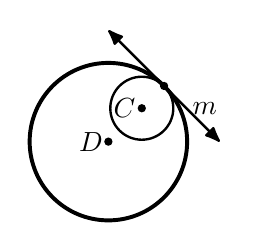
\begin{tikzpicture}[ 
remember picture, %overlay, 
baseline = (current bounding box.south)
] 

\def\radD{1cm}

\def\radC{0.4cm}

\coordinate (d) at (0,0); 

\draw[line width=0.5mm] (d) node[circle, fill=black, inner sep=0pt, outer sep=0pt, minimum size=3pt] {} circle [radius=\radD];

\node(d-label) at ($(d)+(180:0.22*\radD)$) {$  D$};

\draw ($(d)+(45:\radD)$) node[circle, fill=black, inner sep=0pt, outer sep=0pt, minimum size=3pt] (int) {} [];

\draw[line width=0.3mm, ->, >={Latex[round]}] (int) -- ($(int)!1!-90:(d)$);

\draw[line width=0.3mm, ->, >={Latex[round]}] (int) -- ($(int)!1!90:(d)$);

\node (c) at ($(int)!0.4!0:(d)$) {};

\draw[line width=0.3mm] (c) node[circle, fill=black, inner sep=0pt, outer sep=0pt, minimum size=3pt] {} circle [radius=\radC];

\node(c-label) at ($(c)+(180:0.22*\radD)$) {$  C$};

\node(m-label) at ($(c)+(0:0.8*\radD)$) {$  m$};

\end{tikzpicture}

\end{multicols}}
\end{minipage}}
\end{center}  
}

\def \PracticeTwoDayC {\def\currentdir{/storage/emulated/0/Documents/documents/latex/1920/Grade-10/2nd/tangent-lines-and-tangent-circles}

\vspace*{0.3cm}
\begin{center}
\scalebox{0.5}{
\noindent\begin{minipage}{0.3\textwidth}

{\begin{multicols}{2}
3. \hspace*{1.5cm}
\begin{tikzpicture}[
remember picture, overlay, 
baseline = (current bounding box.west)
]  

\def\radE{0.5cm}

\def\radF{0.7cm}

\coordinate (intE) at (0,0); 

\coordinate (intF) at (1.5*\radF,0); 

\node(e) at ($(intE)+(90:\radE)$) {};

\draw[line width=0.5mm] (e) node[circle, fill=black, inner sep=0pt, outer sep=0pt, minimum size=3pt] {} circle [radius=\radE];

\node(e-label) at ($(e)+(50:0.3*\radF)$) {$  E$};

\draw[line width=0.3mm, <->, >={Latex[round]}] ($(intE) +(180:1.2*\radE)$) -- ($(intF) +(0:1.2*\radF)$);

\node(f) at ($(intF)+(-90:\radF)$) {};

\node(n) at ($(intF)+(15:1cm)$) {$  n$};

\draw[line width=0.5mm] (f) node[circle, fill=black, inner sep=0pt, outer sep=0pt, minimum size=3pt] {} circle [radius=\radF];

\node(f-label) at ($(f)+(-50:0.3*\radF)$) {$  F$};

\end{tikzpicture}

 %& 
4. \hspace*{1.5cm}\begin{tikzpicture}[remember picture, overlay, 
baseline = (current bounding box.north)
]  
 
\pgfmathsetmacro{\rone}{1} 

\pgfmathsetmacro{\rtwo}{0.6}
 
\pgfmathsetmacro{\mid}{\rone/(\rone + \rtwo)} 

\pgfmathsetmacro{\out}{\rone/(\rone - \rtwo)} 

\node[draw,circle,minimum size=2 * \rone cm,inner sep=0pt, line width=0.5mm] (c1) at (2*\rone,0) {}; 

\node[draw,circle,minimum size=2 * \rtwo cm,inner sep=0pt, line width=0.5mm] (c2) at (0,0) {}; 

\path (c1.center) -- node[coordinate,pos=\mid] (mid) {} (c2.center); 

\path (c1.center) -- node[coordinate,pos=\out] (out) {} (c2.center); 

\draw(c1.center) node  [circle, fill=black, inner sep=0pt, outer sep=0pt, minimum size=3pt] () {};

\draw(c2.center) node  [circle, fill=black, inner sep=0pt, outer sep=0pt, minimum size=3pt] () {};

\node(i-label) at ($(c1.center)+(180:0.22*\rone)$) {$  I$};

\node(h-label) at ($(c2.center)+(180:0.22*\rone)$) {$  H$};

\foreach \i in {1,2} 
\foreach \j in {1,2} 
\foreach \k in {mid,out} 
\coordinate (t\i\j\k) at (tangent cs:node=c\i,point={(\k)},solution=\j); 

\foreach \i in {1,2} 
\foreach \k in {mid,out} 
\draw[line width=0.3mm, <->, >={Latex[round]}] ($(t1\i\k)!-1cm!(t2\i\k)$) -- ($(t2\i\k)!-0.8cm!(t1\i\k)$); 

\node(p-label) at ($(t21mid)!-1cm!(t11mid)+(110:3pt) $) {$  p$};

\node(s-label) at ($(t22mid)!-1cm!(t12mid)+(-110:3pt) $) {$  s$};

\node(r-label) at ($(t21out)!-1cm!(t11out)+(-70:0.25*\rone) $) {$  r$};

\node(q-label) at ($(t22out)!-1cm!(t12out)+(70:0.25*\rone) $) {$  q$};

\end{tikzpicture}

 %\\
\end{multicols}}
\end{minipage}}
\end{center}   

\vspace*{1.3cm}
B. In $\odot{O}$, $\overline{CT}$, $\overline{ET}$ are tangent segments and $m$ is tangent to $\odot{O}$ at S. 
\begin{center}
\vspace*{-2ex}
\scalebox{0.5}{
\noindent\begin{minipage}{0.3\textwidth}
{
\begin{enumerate}[label = \arabic*. ]
\item $m\angle{OCT}=$ \blank. 
\item $m\angle{OSI}=$ \blank. %\hspace*{8cm}
\begin{tikzpicture}[remember picture, overlay
]

\def\rad{1.2cm}

\node[draw,circle,minimum size=2*\rad,inner sep=0pt, line width=0.5mm, outer sep=0] (c1) at (0,0) {}; 

\node(o-label) at ($(c1.center)+(150:0.22*\rad)$) {$  O$};

\coordinate (t) at (0,-3*\rad); 

\node(t-label) at ($(t)+(270:0.22*\rad)$) {$  T$};

\draw[line width=0.3mm] (c1.center) -- (tangent cs:node=c1, point={(t)}, solution=1) -- (t) -- (tangent cs:node=c1, point={(t)}, solution=2) -- cycle; 

\node(e-label) at ($(tangent cs:node=c1, point={(t)}, solution=1)+(-20:0.2*\rad)$) {$  E$};

\node(c-label) at ($(tangent cs:node=c1, point={(t)}, solution=2)+(200:0.2*\rad)$) {$  C$};

\coordinate (n) at (90:\rad); 

\node(n-label) at ($(n)+(90:0.2*\rad)$) {$  N$};

\coordinate (s) at (-90:\rad); 

\node(s-label) at ($(s)+(-90:0.2*\rad)$) {$  S$};

\node[circle, fill=black, inner sep=0pt, outer sep=0pt, minimum size=3pt] (i) at ($(s)+(180:\rad)$) {};

\coordinate (l) at ($(s)+(180:1.2*\rad)$); 

\node(i-label) at ($(i)+(90:0.2*\rad)$) {$  I$};

\coordinate (m) at ($(s)+(0:1.2*\rad)$); 

\node(l-label) at ($(m)+(90:0.2*\rad)$) {$m$};

\draw[line width=0.3mm] (n) -- (s); 

\draw[line width=0.3mm, <->, >={Latex[round]}] (l) -- (m); 

\end{tikzpicture}
 \vspace*{-2.5ex}
\item If $\overline{SN}=24$ units,  then $\overline{OE}=$ \blank. 
\item If $\overline{OS}=5$ units and $\overline{SI}=12$ units,\newline then $\overline{OI}=$ \blank. 
\item If $\overline{CT}=15$ units,  then $\overline{ET}=$ \blank. 
\item If $\overline{OC}=8$ units and\newline $\overline{ET}=15$ units,  then $\overline{OT}=$ \blank. 
\item If $\overline{OE}=11$ units, then $\overline{NS}=$ \blank. 
\item If $\overline{OS}=7$ units and  $\overline{OT}=25$ units,\newline then $\overline{CT}=$ \blank. 
\end{enumerate}  

\vspace*{-5cm}\hspace*{8.5cm}
\begin{tikzpicture}[remember picture, overlay
]

\def\rad{1.2cm}

\node[draw,circle,minimum size=2*\rad,inner sep=0pt, line width=0.5mm, outer sep=0] (c1) at (0,0) {}; 

\node(o-label) at ($(c1.center)+(150:0.22*\rad)$) {$  O$};

\coordinate (t) at (0,-3*\rad); 

\node(t-label) at ($(t)+(270:0.22*\rad)$) {$  T$};

\draw[line width=0.3mm] (c1.center) -- (tangent cs:node=c1, point={(t)}, solution=1) -- (t) -- (tangent cs:node=c1, point={(t)}, solution=2) -- cycle; 

\node(e-label) at ($(tangent cs:node=c1, point={(t)}, solution=1)+(-20:0.2*\rad)$) {$  E$};

\node(c-label) at ($(tangent cs:node=c1, point={(t)}, solution=2)+(200:0.2*\rad)$) {$  C$};

\coordinate (n) at (90:\rad); 

\node(n-label) at ($(n)+(90:0.2*\rad)$) {$  N$};

\coordinate (s) at (-90:\rad); 

\node(s-label) at ($(s)+(-90:0.2*\rad)$) {$  S$};

\node[circle, fill=black, inner sep=0pt, outer sep=0pt, minimum size=3pt] (i) at ($(s)+(180:\rad)$) {};

\coordinate (l) at ($(s)+(180:1.2*\rad)$); 

\node(i-label) at ($(i)+(90:0.2*\rad)$) {$  I$};

\coordinate (m) at ($(s)+(0:1.2*\rad)$); 

\node(l-label) at ($(m)+(90:0.2*\rad)$) {$m$};

\draw[line width=0.3mm] (n) -- (s); 

\draw[line width=0.3mm, <->, >={Latex[round]}] (l) -- (m); 

\end{tikzpicture}
 \vspace*{5cm}
}
\end{minipage}}
\end{center}  
}

\def \MasteryDayC {\def\currentdir{/storage/emulated/0/Documents/documents/latex/1920/Grade-10/2nd/tangent-lines-and-tangent-circles}

\def\myrad{1cm}

\textbf{Problem Set}

\vspce

Use the given figures to find the values of $x$ and $y$.

\begin{center}
\scalebox{0.5}{
\noindent\begin{minipage}{0.3\textwidth}
{\begin{tabularx}{\textwidth}{XXX}
1. \begin{tikzpicture}[dot/.style={circle, fill=black, inner sep=0pt, outer sep=0pt, minimum size=3pt}]

\node[draw,circle,minimum size=2*\myrad,inner sep=0pt, line width=0.5mm, outer sep=0] (o) at (0,0) {}; 

\node(o-dot)[dot] at (o.center) {};

\node(o-label) at ($(o.center)+(180:0.27*\myrad)$) {$  O$};

\coordinate (t) at (2*\myrad,0); 

\node(58) at ($(t)+(190:0.5*\myrad)$) {$  58\degree$};

\draw[line width=0.3mm] (o.center) -- (tangent cs:node=o, point={(t)}, solution=1) -- (t) -- (tangent cs:node=o, point={(t)}, solution=2) -- cycle; 

\node(x-label) at ($(o)+(0:0.22*\myrad)$) {$  x$};

\end{tikzpicture}

 & 4. \begin{tikzpicture}[dot/.style={circle, fill=black, inner sep=0pt, outer sep=0pt, minimum size=3pt}]

\node[draw,circle,minimum size=2*\myrad,inner sep=0pt, line width=0.5mm, outer sep=0] (c1) at (0,0) {};

\node(o-dot)[dot] at (o.center) {};

\coordinate (a) at ($(o.center)+(90:\myrad) $); 

\coordinate (b) at ($(o.center)+(-90:\myrad) $); 

\coordinate (c) at ($(o.center)+(180:\myrad) $); 

\coordinate (ext) at ($(b)+(180:2*\myrad) $); 

\node(o-label) at ($(o.center)+(20:0.23*\myrad)$) {$  O$};

\node(x-label) at ($(a)+(-112:0.38*\myrad)$) {$  x$};

\node(y.label) at ($(b)+(150:0.48*\myrad)$) {\tiny $y$};

\node(45-label) at ($(ext)+(20:0.6*\myrad)$) {$  45\degree$};

\draw[line width=0.3mm] (b) -- (c) -- (ext) -- (b) -- (a) ; 

\draw[line width=0.3mm] (a) -- (c) ; 

\end{tikzpicture}

 & 7. \begin{tikzpicture}[dot/.style={circle, fill=black, inner sep=0pt, outer sep=0pt, minimum size=3pt}, dim-label/.style={fill=white, rectangle, inner sep=2pt, outer sep=0pt}]

\node[draw,circle,minimum size=2*\myrad,inner sep=0pt, line width=0.5mm, outer sep=0] (e) at (0,0) {};

\node(e-dot)[dot] at (e.center) {};

\coordinate (k) at ($(e.center) +(90:\myrad)$);

\node(k-label) at ($(k)+(90:0.18*\myrad)$) {$  K$};

\coordinate (a) at ($(e.center) + (180:\myrad)$);

\node(a-label) at ($(a)+(180:0.18*\myrad)$) {$  A$};

\coordinate (r) at ($(e.center) +(-90:\myrad)$);

\node(r-label) at ($(r)+(-90:0.18*\myrad)$) {$  R$};

\coordinate (g) at ($(a)+(90:\myrad) $);

\node(g-label) at ($(g)+(90:0.18*\myrad)$) {$  G$};

\coordinate (d) at ($(a)+(-90:\myrad) $);

\node(d-label) at ($(d)+(-90:0.18*\myrad)$) {$  D$};

\coordinate (o) at ($(k)+(0:1.3*\myrad) $);

\node(o-label) at ($(o)+(50:0.18*\myrad)$) {$  O$};

\coordinate (ext) at ($(a)+(180:0.4*\myrad) $);

\coordinate (u) at (tangent cs:node=e, point={(o)}, solution=2); 

\node(u-label) at ($(u)+(-40:0.22*\myrad)$) {$  U$};

\coordinate (guess1) at ($(o)!1.7!(u)$);

\coordinate (guess2) at ($(d)!1.88!(r)$);

\node(e-label) at ($(e.center)+(20:0.18*\myrad)$) {$  E$};

\draw[line width=0.3mm] (u) -- (o) -- (g) -- (d) -- (r);

\path[name path=line1.guess, line width=0.3mm] (u) -- (guess1); 

\path[name path=line2.guess, line width=0.3mm] (r) -- (guess2); 

\fill[red, name intersections={of=line1.guess and line2.guess, name=point}];

\draw[line width=0.3mm] (u) -- (point-1) -- (r) ; 

\node(l-label) at ($(point-1)+(-60:0.18*\myrad)$) {$  L$};

\draw[{Rays[n=2].Classical TikZ Rightarrow[]}-{Classical TikZ Rightarrow[].Rays[n=2]}, line width=0.3mm] ($(ext)+(90:\myrad+1pt)$) -- ($(ext)+(-90:\myrad+1pt)$);

\node[dim-label] (x-label) at ($(ext)+(90:0.3*\myrad)$) {\tiny $\text{x cm}$};

\node (8cm) at ($(g)+(20:0.5*\myrad)$) {\tiny 8 cm};

\node (16cm) at ($(o)+(-65:0.5*\myrad)$) {\tiny 16 cm};

\node (6cm) at ($(u)+(-70:0.5*\myrad)$) {\tiny 6 cm};

\node (12cm) at ($(r)+(200:0.5*\myrad)$) {\tiny 12 cm};
\end{tikzpicture}

 \\[-3ex]

2. \begin{tikzpicture}[dot/.style={circle, fill=black, inner sep=0pt, outer sep=0pt, minimum size=3pt}]

\node[draw,circle,minimum size=2*\myrad, inner sep=0pt, line width=0.5mm, outer sep=0] (o) at (0,0) [] {};

\node(o-dot)[dot] at (o.center) {};

\coordinate (ext) at ($(o.center)+(200:2*\myrad) $); 

\node(o-label) at ($(o.center)+(18:0.23*\myrad)$) {$  O$};

\node(42-label) at ($(ext)+(25:0.6*\myrad)$) {$  42\degree$};

\draw[line width=0.3mm] ($(tangent cs:node=o, point={(ext)}, solution=2)!2!0:(o.center)$) -- (ext) -- (tangent cs:node=o, point={(ext)}, solution=2) -- (o.center) ; 

\draw[line width=0.3mm] (o.center) -- ($(tangent cs:node=o, point={(ext)}, solution=2)!2!0:(o.center)$) ; 

\node(x-label) at ($(tangent cs:node=o, point={(ext)}, solution=2)!2!0:(o.center) + (163:0.5*\myrad) $) {$  x$};


\end{tikzpicture}

 & 5. \begin{tikzpicture}[dot/.style={circle, fill=black, inner sep=0pt, outer sep=0pt, minimum size=3pt}]

\node[draw,circle,minimum size=2*\myrad,inner sep=0pt, line width=0.5mm, outer sep=0] (c1) at (0,0) {};

\node(o-dot)[dot] at (o.center) {};

\coordinate (ext) at ($(o.center)+(0:2.4*\myrad) $); 

\node(o-label) at ($(o.center)+(180:0.22*\myrad)$) {$  O$};

\node(x-label) at ($(tangent cs:node=o, point={(ext)}, solution=1)+(-60:0.25*\myrad)$) {\tiny $x$};

\node(y-label) at ($(o.center)+(32:0.22*\myrad)$) {\tiny $y$};

\node(z-label) at ($(tangent cs:node=o, point={(ext)}, solution=2)+(60:0.25*\myrad)$) {\tiny $z$};

\node(35-label) at ($(ext)+(169:0.88*\myrad)$) {\tiny $35\degree$};

\draw[line width=0.3mm] (ext) -- (o.center) -- (tangent cs:node=o, point={(ext)}, solution=1) ; 

\draw[line width=0.3mm] (tangent cs:node=o, point={(ext)}, solution=1) -- (tangent cs:node=o, point={(ext)}, solution=2) ; 

\draw[line width=0.3mm] (tangent cs:node=o, point={(ext)}, solution=2) -- (o.center) ; 

\draw[line width=0.3mm] ($(ext)!1.5!(tangent cs:node=o, point={(ext)}, solution=1)$) -- (ext) -- ($(ext)!1.5!(tangent cs:node=o, point={(ext)}, solution=2)$); 

\end{tikzpicture}

 & 8. \begin{tikzpicture}[dot/.style={circle, fill=black, inner sep=0pt, outer sep=0pt, minimum size=3pt}]

\node[draw,circle,minimum size=2*\myrad,inner sep=0pt, line width=0.5mm, outer sep=0] (o) at (0,0) {};

\node(o-dot)[dot] at (o.center) {};

\coordinate (a) at ($(o.center)+(-90:\myrad) $); 

\coordinate (ext) at ($(a)+(180:2*\myrad) $); 

\node(o-label) at ($(o.center)+(20:0.22*\myrad)$) {$  O$};

\node(x1-label) at ($(o.center)+(190:0.5*\myrad)$) {$x$};

\node(x2-label) at ($(o.center)+(-70:0.5*\myrad)$) {$x$};

\node(4) at ($(o.center)+(200:1.6*\myrad)$) {$  4$};

\node(8) at ($(a)+(190:\myrad)$) {$8$};

\draw[line width=0.3mm] (ext) -- (tangent cs:node=o, point={(ext)}, solution=1) -- (o.center) -- cycle; 

\end{tikzpicture}
 \\[-6ex]

3. \begin{tikzpicture}[dot/.style={circle, fill=black, inner sep=0pt, outer sep=0pt, minimum size=3pt}]

\node[draw,circle,minimum size=2*\myrad,inner sep=0pt, line width=0.5mm, outer sep=0] (o) at (0,0) {};

\node(o-dot)[dot] at (o.center) {};

\coordinate (ext) at ($(o.center)+(270:2*\myrad) $); 

\node(o-label) at ($(o.center)+(20:0.23*\myrad)$) {$  O$};

\node(x-label) at ($(ext)+(75:0.5*\myrad)$) {$  x$};

\node[rotate=-30](60-label) at ($(o.center)+(-50:0.5*\myrad)$) {$ 60\degree$};


\draw[line width=0.3mm] (ext) -- (tangent cs:node=o, point={(ext)}, solution=1) -- (o.center) -- cycle; 

\end{tikzpicture}

 & 6. \begin{tikzpicture}[dot/.style={circle, fill=black, inner sep=0pt, outer sep=0pt, minimum size=3pt}, dim-label/.style={fill=white, rectangle, inner sep=2pt, outer sep=0pt}]

\node[draw,circle,minimum size=2*\myrad,inner sep=0pt, line width=0.5mm, outer sep=0] (o) at (0,0) {};

\node(o-dot)[dot] at (o.center) {};

\coordinate(a) at ($(o.center) +(-90:\myrad)$);

\coordinate(b) at ($(o.center) + (0:\myrad)$);

\coordinate (ext) at ($(a)+(180:\myrad)$); 

\coordinate (ext2) at ($(b)+(90:\myrad)$); 

\coordinate (ext3) at ($(ext)+(90:2*\myrad)$); 

\coordinate (ext4) at ($(ext)+(0:2*\myrad)$); 

\coordinate (ext5) at ($(b)+(0:0.3*\myrad)$); 

\draw[line width=0.3mm] (ext) rectangle (ext2);

\begin{scope} [rotate=0]
\draw[line width=0.3mm] (ext) rectangle ++(0.22*\myrad,0.22*\myrad) node[transform shape]{};
\end{scope}

\begin{scope} [rotate=180]
\draw[line width=0.3mm] (ext2) rectangle ++(0.22*\myrad,0.22*\myrad) node[transform shape]{};
\end{scope}

\begin{scope} [rotate=-90]
\draw[line width=0.3mm] (ext3) rectangle ++(0.22*\myrad,0.22*\myrad) node[transform shape]{};
\end{scope}

\begin{scope} [rotate=90]
\draw[line width=0.3mm] (ext4) rectangle ++(0.22*\myrad,0.22*\myrad) node[transform shape]{};
\end{scope}

\node(o-label) at ($(o.center)+(180:0.23*\myrad)$) {$  O$};

\draw[line width=0.3mm] (o.center) -- (b) ;

\node(14) at ($(o.center)+(15:0.5*\myrad)$) {\tiny $\text{14 ft.}$}; 

\draw[{Rays[n=2].Classical TikZ Rightarrow[]}-{Classical TikZ Rightarrow[].Rays[n=2]}, line width=0.3mm] ($(ext5)+(90:\myrad+1pt)$) -- ($(ext5)+(-90:\myrad+1pt)$);

\node[dim-label] (x-label) at (ext5) {\tiny $\text{x ft.}$};

\end{tikzpicture}

 & \vspace*{-2cm} 9.\hspace*{1.5cm}\begin{tikzpicture}[dot/.style={circle, fill=black, inner sep=0pt, outer sep=0pt, minimum size=3pt}, 
remember picture, overlay, 
baseline = (current bounding box.south)
]  

\node[draw,circle,minimum size=2*\myrad,inner sep=0pt, line width=0.5mm, outer sep=0] (o) at (0,0) {};

\node(o-dot)[dot] at (o.center) {};

\coordinate (a) at ($(o.center)+(-90:\myrad) $); 

\coordinate (ext) at ($(a)+(0:2*\myrad) $); 

\node(o-label) at ($(o.center)+(90:0.22*\myrad)$) {$  O$};

\node(5) at ($(o.center)+(250:0.45*\myrad)$) {$  5$};

\node(x) at ($(o.center)+(-20:1.5*\myrad)$) {$x$};

\node(12) at ($(a)+(-10:1.1*\myrad)$) {$  12$};

\draw[line width=0.3mm] (ext) -- (tangent cs:node=o, point={(ext)}, solution=2) -- (o.center) -- cycle; 

\end{tikzpicture}


%\end{minipage} 
\\%[-2ex]

\end{tabularx}} 
\end{minipage}}
\end{center}


}



\def \EvaluationDayC {
\input{/storage/emulated/0/Documents/documents/latex/1920/Grade-10/2nd/tangent-lines-and-tangent-circles/qz-tangent-lines-and-tangent-circles-input} 
}

\def \RemediationDayC {}

\def \LessonDayD {Angles Formed by Secants and Tangents}

\def \LearningCompetenciesDayD {}

\def \ObjectivesDayD {
\item %cogverbstart
Describe
%cogverbend
the angles formed by secants and tangents; 
\item %psyverbstart
Find
%psyverbend
the angles formed by secants and tangents to determine whether a binomial is a factor of a given polynomial; and, 
\item %affverbstart
Show
%affverbend
%valsstart
independence and willingness
%valsend
in solving problems.
}

\def \PurposeDayD {The purpose of this lesson is to enable the students to solve real life problems involving the angles formed by secants and tangents.}  

\def \ApplicationDayD { Let the students answer the following questions: 
\begin{enumerate}[label = \arabic*. ]
%1
\item In what real life situations or problems can we observe some examples of angles formed by secants and tangents? 
%2
\item How can you apply your knowledge of angles formed by secants and tangents in solving these real life problems? 

\end{enumerate}   
}

\def \GeneralizationDayD {Let the students answer the following questions: 
\begin{enumerate}[label = \arabic*. ]
%1
\item In your own words, what is the angles formed by secants and tangents? 
%2
\item How do we solve problems involving angles formed by secants and tangents? 

\end{enumerate}   
}

\def \TeachersGuideDayD {pp. 141--144}

\def \LMPagesDayD {pp. 130--133}

\def \TextbookPagesDayD {pp. 140--144}

\def \AdditionalMaterialsDayD {}

\def \OtherResourcesDayD {Flashcards}

\def \ReviewDayD {\begin{center}
\textbf{Angles Formed by Secants and Tangents}
\end{center}

\vspace*{1ex}

\begin{center}
\vspace*{-2ex}
\scalebox{0.5}{
\noindent\begin{minipage}{0.3\textwidth}
{
\textbf{Intersecting Secants -- Exterior Theorem:} The measure of an angle formed by two secants that intersect in the exterior of a circle is one-half the difference of its intercepted arcs. 

\vspce 

\textbf{Tangent Point -- Secant Theorem:}  The measure of an angle formed by a tangent and a secant drawn at the point of contact is one-half the measure of its intercepted arc. 

\vspce 

\textbf{Intersecting Secants -- Interior  Theorem:} The measure of an angle formed by two secants intersecting in the interior of the circle is equal to one-half the sum of the measures of its intercepted arcs. 
}
\end{minipage}}
\end{center} 
 }



\def \ExamplesDayD {}

\def \PracticeOneDayD {\def\radA{1cm}
\def\curdir{/storage/emulated/0/Documents/documents/latex/1920/Grade-10/2nd/angles-formed-by-secants-and-tangents}

\textbf{Practice Exercises}

\vspce

Find the value of $x$. 

\begin{center}
\scalebox{0.5}{
\noindent\begin{minipage}{0.3\textwidth}
{\begin{tabularx}{\textwidth}{XX}
1. \begin{tikzpicture}[dot/.style={circle, fill=black, inner sep=0pt, outer sep=0pt, minimum size=3pt}, baseline = (current bounding box.west)]

\node[draw,circle,minimum size=2*\radA, inner sep=0pt, line width=0.5mm, outer sep=0] (circ) at (0,0) {};

\coordinate (a) at ($(circ) + (120:\radA)$);

\coordinate (b) at ($(circ) + (-60:\radA)$);

\coordinate (c) at ($(circ) + (70:\radA)$);

\coordinate (d) at ($(circ) + (200:\radA)$);

\draw[name path=line1, line width=0.3mm] (a)--(b);

\draw[name path=line2, line width=0.3mm] (c)--(d);

\fill[black, name intersections={of=line1 and line2, name=point}];

\node[dot] (x) at (point-1){};

\node(37-label) at ($(x)+(80: 0.85*\radA)$) {$  37\degree$};

\node(x.label) at ($(x)+(85:0.22*\radA)$) {$  x$};

\node(105.label) at ($(circ)+(-110:1.3*\radA)$) {$  105\degree $};

\end{tikzpicture} 
 & 5. \begin{tikzpicture}[dot/.style={circle, fill=black, inner sep=0pt, outer sep=0pt, minimum size=3pt}, baseline = (current bounding box.west)]

\node[draw,circle,minimum size=2*\radA, inner sep=0pt, line width=0.5mm, outer sep=0] (circ) at (0,0) {};

\coordinate (a) at ($(circ) + (50: 1.4*\radA)$);

\coordinate (b) at ($(circ) + (215: 1.8*\radA)$);

\coordinate (c) at ($(circ) + (-25: 1.4*\radA)$);

\node(x.label) at ($(b)+(23:0.44*\radA)$) {$  x$};

\node(80.label) at ($(circ)+(5:0.7*\radA)$) {$  80\degree $};

\node(140.label) at ($(circ)+(130:1.25*\radA)$) {$  140\degree $};

\node(130.label) at ($(circ)+(-80:1.2*\radA)$) {$  130\degree $};

\draw[line width=0.3mm, <->, >={Latex[round]}] (a) -- (b) -- (c) ;

\end{tikzpicture} 

 \\
 
2. \begin{tikzpicture}[dot/.style={circle, fill=black, inner sep=0pt, outer sep=0pt, minimum size=3pt}, baseline = (current bounding box.west)]

\node[draw,circle,minimum size=2*\radA, inner sep=0pt, line width=0.5mm, outer sep=0] (circ) at (0,0) {};

\coordinate (a) at ($(circ) + (\radA, 0)$);

\coordinate (b) at ($(circ) + (110:\radA)$);

\coordinate (c) at ($(a) + (0, -\radA)$);

\pic [draw, line width=0.3mm, angle radius=0.4*\radA, "$x$"] {angle=b--a--c};

\draw[line width=0.3mm] (b)--(a);

\draw[line width=0.3mm, <->, >={Latex[round]}] (c)--($(a)!-1!(c) $);

\node(250-label) at ($(circ)+(-120:1.35*\radA)$) {$  250\degree $};

\end{tikzpicture} 
 & 6. \begin{tikzpicture}[dot/.style={circle, fill=black, inner sep=0pt, outer sep=0pt, minimum size=3pt}, baseline = (current bounding box.west)]

\node[draw,circle,minimum size=2*\radA, inner sep=0pt, line width=0.5mm, outer sep=0] (circ) at (0,0) {};

\coordinate (a) at ($(circ) + (150: 1.4*\radA)$);

\coordinate (b) at ($(circ) + (-17: 1.4*\radA)$);

\coordinate (c) at ($(circ) + (27: 1.4*\radA)$);

\coordinate (d) at ($(circ) + (200: 1.4*\radA)$);

\draw[name path=line1, line width=0.3mm, <->, >={Latex[round]}] (a) -- (b);

\draw[name path=line2, line width=0.3mm, <->, >={Latex[round]}] (c) -- (d);

\fill[black, name intersections={of=line1 and line2, name=point}];

\node[dot] (int) at (point-1){};

\node(x.label) at ($(int)+(0:0.35*\radA)$) {$  x$};

\node(40-label) at ($(int)+(0:1.2*\radA)$) {$  40\degree $};

\node(60-label) at ($(int)+(180:1.4*\radA)$) {$  60\degree $};

\end{tikzpicture} 
 \\

3. \begin{tikzpicture}[dot/.style={circle, fill=black, inner sep=0pt, outer sep=0pt, minimum size=3pt}, baseline = (current bounding box.west)]

\node[draw,circle,minimum size=2*\radA, inner sep=0pt, line width=0.5mm, outer sep=0] (circ) at (0,0) {};

\coordinate (a) at ($(circ) + (35:1.4*\radA)$);

\coordinate (b) at ($(circ) + (180:2*\radA)$);

\coordinate (c) at ($(circ) + (-30:1.4*\radA)$);

\node(x.label) at ($(b)+(0:0.5*\radA)$) {$  x$};

\node(24.label) at ($(circ)+(180:0.65*\radA)$) {$ 24\degree $};

\node(118.label) at ($(circ)+(0:0.6*\radA)$) {$ 118\degree $};

\draw[line width=0.3mm, <->, >={Latex[round]}] (a) -- (b) -- (c) ;

\end{tikzpicture} 

 & 7. \begin{tikzpicture}[dot/.style={circle, fill=black, inner sep=0pt, outer sep=0pt, minimum size=3pt}, baseline = (current bounding box.west)
]

\node[draw,circle,minimum size=2*\radA, inner sep=0pt, line width=0.5mm, outer sep=0] (circ) at (0,0) {};

\coordinate (a) at ($(circ) + (120: \radA)$);

\coordinate (b) at ($(circ) + (290: \radA)$);

\coordinate (c) at ($(circ) + (40: \radA)$);

\coordinate (d) at ($(circ) + (240: \radA)$);

\node(78.label) at ($(circ)+(80:1.25*\radA)$) {$  78\degree $};

\node(28.label) at ($(circ)-(87:1.25*\radA)$) {$  28\degree $};

\draw[line width=0.3mm, name path=line1] (a) -- (b);

\draw[line width=0.3mm, name path=line2] (c) -- (d);

\fill[black, name intersections={of=line1 and line2, name=point}];

\node[dot] (int) at (point-1){};

\node(x.label) at ($(int)+(160:0.6*\radA)$) {\tiny $\text{x+53}\degree$};

\pic [draw, line width=0.2mm, angle radius=0.25*\radA] {angle=a--int--d};


\end{tikzpicture} 


 \\

4. \begin{tikzpicture}[dot/.style={circle, fill=black, inner sep=0pt, outer sep=0pt, minimum size=3pt}, baseline = (current bounding box.west)]

\node[draw,circle,minimum size=2*\radA, inner sep=0pt, line width=0.5mm, outer sep=0] (circ) at (0,0) {};

\coordinate (ext) at ($(circ) + (-90:1.7*\radA)$);

\node(x.label) at ($(ext)+(90:0.22*\radA)$) {$x$};

\node[dot] (tan1) at (tangent cs:node=circ, point={(ext)}, solution=1) {}; 

\node[dot] (tan2) at (tangent cs:node=circ, point={(ext)}, solution=2) {}; 

\node(135.label) at ($(circ)+(-90:0.75*\radA) $) {$135\degree  $};

\draw[line width=0.3mm, <->, >={Latex[round]}] ($(tan2)!-0.6!(ext) $) -- (ext) -- ($(tan1)!-0.6!(ext) $) ;

\end{tikzpicture} 

 & 8. \begin{tikzpicture}[dot/.style={circle, fill=black, inner sep=0pt, outer sep=0pt, minimum size=3pt}, baseline = (current bounding box.west)]

\node[draw,circle,minimum size=2*\radA, inner sep=0pt, line width=0.5mm, outer sep=0] (circ) at (0,0) {};

\coordinate (a) at ($(circ) + (120: \radA)$);

\coordinate (b) at ($(circ) + (-120: \radA)$);

\coordinate (c) at ($(circ) + (200: \radA)$);

\coordinate (d) at ($(circ) + (-20: \radA)$);

\node(1-label) at ($(circ)+(50:1.3*\radA)$) {$50x$};

\node(2-label) at ($(circ)+(210:1.55*\radA)$) {$  \text{2x+24}\degree $};

\draw[line width=0.3mm, name path=line1] (a) -- (b);

\draw[line width=0.3mm, name path=line2] (c) -- (d);

\fill[black, name intersections={of=line1 and line2, name=point}];

\node[dot] (int) at (point-1){};

\begin{scope} [rotate=0]
\draw[line width=0.3mm] (int) rectangle ++(0.22*\radA,0.22*\radA) node[transform shape]{};
\end{scope}

\end{tikzpicture} 

 \\

\end{tabularx}}
\end{minipage}}
\end{center} 
  }

\def \PracticeTwoDayD {\input{/storage/emulated/0/Documents/documents/latex/1920/Grade-10/2nd/angles-formed-by-secants-and-tangents/ps-angles-formed-by-secants-and-tangents-input2-dll}
}

\def \MasteryDayD {\def\curdir{/storage/emulated/0/Documents/documents/latex/1920/Grade-10/2nd/angles-formed-by-secants-and-tangents}
\def\radA{1cm}
\def\radB{1cm}

\textbf{Problem Set}

\vspce 

%\begin{enumerate}[label = \Alph*. ]
%\item \hspce 
A. Use the figure to solve the following. 
\begin{center}
\vspace*{2ex}
\scalebox{0.5}{
\noindent\begin{minipage}{0.3\textwidth}
{
\begin{enumerate}[label = \arabic*. ]
%1
\item If $m\arc{AC}=40\degree $ and $m\arc{BD}=80\degree $, find $m\angle{ATC} $. 
%2
\item If $m\angle{BTC} =142\degree $ and $m\arc{AD}=156\degree $, find $m\arc{BC}$. 
%3
\item If $m\arc{ADB} =208\degree $, $m\arc{AC} =52\degree $ and $m\arc{DBC}=192\degree $, find $m\angle{ATD}$.

\begin{center}

\hspace*{-40pt}\begin{tikzpicture}[dot/.style={circle, fill=black, inner sep=0pt, outer sep=0pt, minimum size=3pt}]

\node(circ) at (0,0) {};

\draw[line width=0.5mm] (circ) circle (\radA);

\coordinate (d) at ($(circ) + (50:\radA)$); 

\coordinate (c) at ($(circ) + (220:\radA)$);

\coordinate (a) at ($(circ) + (175:\radA)$);

\coordinate (b) at ($(circ) + (-40:\radA)$);

\draw[name path=line1, line width=0.3mm, <->, >={Latex[round]}] ($(a)!-35pt!(b) $) -- ($(b)!-0.66*\radA!(a) $);

\draw[name path=line2, line width=0.3mm, <->, >={Latex[round]}] ($(c)!-35pt!(d) $) -- ($(d)!-0.66*\radA!(c) $);

\fill[black, name intersections={of=line1 and line2, name=point}];

\node[dot] (int) at (point-1){};

\node(t.label) at ($(int)+(90:0.22*\radA)$) {$  T$};

\node(d.label) at ($(d)+(90:0.25*\radA)$) {$  D$};

\node(c.label) at ($(c)+(-100:0.25*\radA)$) {$  C$};

\node(a.label) at ($(a)+(120:0.33*\radA)$) {$  A$};

\node(b.label) at ($(b)+(20:0.33*\radA)$) {$  B$};

\end{tikzpicture} 
 

\end{center} 

\end{enumerate} 
}
\end{minipage}}
\end{center} 

%\item \hspce
B. Solve each problem completely.  
\begin{center}
\vspace*{2ex}
\scalebox{0.5}{
\noindent\begin{minipage}{0.3\textwidth}
{
\begin{enumerate}[label = \arabic*. ]
%1
\item The angle formed by two secants intersecting in the exterior of a circle measures $64\degree $. One of the intercepted arcs is $208\degree $. Find the other arc. 
%2
\item In $\odot{Q} $, the endpoints of chord $\overline{OK} $ are the points of tangency of lines $\overleftrightarrow{TO} $ and $\overleftrightarrow{TK}$. If $\triangle{TOK}$ is an equilateral triangle, find $m\arc{OIK}$. 
%3
\item In $\odot{O} $, $\overline{LM} $ is a diameter of $\odot{O} $ where $\overline{OM} $ extends its own length to $P$. If $\overline{PN} $ is a tangent segment to $\odot{O} $ at $N$, find $m\angle{P} $. 

\begin{center}
\begin{tikzpicture}[dot/.style={circle, fill=black, inner sep=0pt, outer sep=0pt, minimum size=3pt}%, remember picture, overlay
]

\node[draw, circle, minimum size=2*\radB,inner sep=0pt, line width=0.5mm, outer sep=0] (q) at (0,0) {};

\node(q.dot)[dot] at (q.center) {};

\node(q.label) at ($(q)+(190:0.22*\radB)$) {$  Q$};

\coordinate (t) at ($(q) + (0:2.2*\radB)$); 

\node(t.label) at ($(t)+(0:0.22*\radB)$) {$  T$};

\node[dot] (i) at ($(q)+(230:\radB)$) {};

\node(i.label) at ($(i)+(230:0.22*\radB)$) {$  I$};

\node[dot] (k) at (tangent cs:node=q, point={(t)}, solution=1) {};

\node(k.label) at ($(k)+(90:0.22*\radB)$) {$  K$};

\node[dot] (o) at (tangent cs:node=q, point={(t)}, solution=2) {};

\node(o.label) at ($(o)+(280:0.22*\radB)$) {$  O$};

\draw[line width=0.3mm, <->, >={Latex[round]}] ($(k)!-\radB!(t)$) -- (t) -- ($(o)!-\radB!(t)$);

\draw[line width=0.3mm] (k) -- (o) ;

\end{tikzpicture}  
 

%\hspace*{-30pt}
\begin{tikzpicture}[dot/.style={circle, fill=black, inner sep=0pt, outer sep=0pt, minimum size=3pt}]

\node[draw, circle, minimum size=2*\radB, inner sep=0pt, line width=0.5mm, outer sep=0] (o) at (0,0) {};

\node(o.dot)[dot] at (o.center) {};

\node(o.label) at ($(o)+(270:0.22*\radB)$) {$  O$};

\coordinate (l) at ($(o) + (-\radB, 0)$); 

\node(l.label) at ($(l)+(180:0.18*\radB)$) {$  L$};

\coordinate (p) at ($(o) + (0:2*\radB)$); 

\node(p.label) at ($(p)+(0:0.22*\radB)$) {$  P$};

\node(m.label) at ($(o)+(0:\radB)+(-40:0.3*\radB)$) {$  M$};

\node[dot] (n) at (tangent cs:node=o, point={(p)}, solution=1) {};

\node(n.label) at ($(n)+(60:0.22*\radB)$) {$  N$};

\draw[line width=0.3mm] (l) -- (p) -- (n) -- (o.center) ;

\begin{scope} [rotate=-120]
\draw[line width=0.3mm] (n) rectangle ++(0.35*\radB,0.35*\radB) node[transform shape]{};
\end{scope}

\end{tikzpicture} 

 

\end{center} 

\end{enumerate} 
}
\end{minipage}}
\end{center} 
%\end{enumerate} }



\def \EvaluationDayD {
\input{/storage/emulated/0/Documents/documents/latex/1920/Grade-10/2nd/angles-formed-by-secants-and-tangents/qz-angles-formed-by-secants-and-tangents-input} 
}

\def \RemediationDayD {}
 


% Start the document
\begin{document}


\begin{center}

{
\setlength\arrayrulewidth{2pt}
%\begin{tabularx}{\textwidth}{|Y|R|L|R|L|}
\begin{tabular}{|p{161pt}|p{163pt}|p{163pt}|p{163pt}|p{163pt}|}

\hline

\multirow[c]{3}{15em}{
\begin{tikzpicture}[remember picture, overlay]
\node (deped) at (15:5mm) {
\includegraphics[width=3.5em]{/storage/emulated/0/Documents/documents/latex/1920/deped2.png}};
\end{tikzpicture}
\centering \textbf{\hspace*{2.5em}\makecell{GRADES 1 to 12 \\ DAILY LESSON LOG}}
}  
& 	
\textbf{School}  & 
\School & 	
\textbf{Grade Level} & 
Grade \Grade 
\\

\cline{2-5}

& \textbf{Teacher} 
& \Teacher 
& \textbf{Learning Area} 
& \Subject \\

\cline{2-5}

& \textbf{Teaching Dates and Time} 
& Week \WeekNum, \LessonWeek 
& \textbf{Quarter} 
& \Quarter \\

\hline

\end{tabular} 
%\end{tabularx} 
}


\begin{longtable}{|p{135pt}|p{135pt}|p{135pt}|p{135pt}|p{135pt}|p{135pt}|}

\hline

\textbf{I. OBJECTIVES } & 	
\thead{DAY 1}  & 
\thead{DAY 2}  & 	
\thead{DAY 3}  & 
\thead{DAY 4}  &
\thead{DAY 5}  \\

\hline

\hspce \textbf{Learning Competencies/ \newline Objectives: %(Write the LC code for each.) 
}
&	

% Day 1 Learning Competencies
\LearningCompetenciesDayA

\begin{enumerate}[leftmargin=1em, nolistsep]

\ObjectivesDayA

\end{enumerate}

&

% Day 2 Learning Competencies

\LearningCompetenciesDayB
 
\begin{enumerate}[leftmargin=1em, nolistsep]

\ObjectivesDayB

\end{enumerate}

& 

% Day 3 Learning Competencies

\LearningCompetenciesDayC
 
\begin{enumerate}[leftmargin=1em, nolistsep]

\ObjectivesDayC

\end{enumerate}

&

% Day 4 Learning Competencies

\LearningCompetenciesDayD
 
 
\begin{enumerate}[leftmargin=1em, nolistsep]

\ObjectivesDayD

\end{enumerate} 

&

% Day 5 Learning Competencies

\LearningCompetenciesDayE
 
 
\begin{enumerate}[leftmargin=1em, nolistsep]

\ObjectivesDayE

\end{enumerate} 

\\

\hline
\multirow[l]{2}{15em}{\textbf{II. CONTENT}} & \Content 
\\

\cline{2-6}

& 
% Day 1 Lesson 
\vspace*{-2em}
\begin{center}
\textbf{\LessonDayA}
\end{center} 

& 
% Day 2 Lesson 
\vspace*{-2em}
\begin{center}
\textbf{\LessonDayB}
\end{center} 

& 
% Day 3 Lesson 
\vspace*{-2em}
\begin{center}
\textbf{\LessonDayC}
\end{center}  

& 
% Day 4 Lesson 
\vspace*{-2em}
\begin{center}
\textbf{\LessonDayD}
\end{center}  

& 
% Day 5 Lesson
\vspace*{-2em} 
\begin{center}
\textbf{\LessonDayE}
\end{center}  

\\
 & & & & &
\\[-2.5em]

\hline

\textbf{III. LEARNING RESOURCES} 
&
\multicolumn{5}{l|}{}
\\
\hline

\hspce \textbf{A. References} & & & & &
\\
\hline

\raggedright\hspce \hspce \textbf{1. Teacher's Guide Pages} & 

% Day 1 Teachers Guide References
\TeachersGuideDayA 

&
% Day 2 Teachers Guide References
\TeachersGuideDayB 

&
% Day 3 Teachers Guide References
\TeachersGuideDayC 

&
% Day 4 Teachers Guide References
\TeachersGuideDayD

&
% Day 5 Teachers Guide References
\TeachersGuideDayE 

\\
\hline

\raggedright\hspce \hspce \textbf{2. Learner's Materials Pages} & 

% Day 1 References
\LMPagesDayA 

&
% Day 2 References
\LMPagesDayB 

&
% Day 3 References
\LMPagesDayC 

&
% Day 4 References
\LMPagesDayD 

&
% Day 5 References
\LMPagesDayE

\\

\hline

\hspce \hspce \textbf{3. Textbook Pages} & 

% Day 1 Textbook Pages 
\TextbookPagesDayA 

& 
% Day 2 Textbook Pages 
\TextbookPagesDayB 

&
% Day 3 Textbook Pages 
\TextbookPagesDayC 

& 
% Day 4 Textbook Pages 
\TextbookPagesDayD

& 
% Day 5 Textbook Pages 
\TextbookPagesDayE 

\\

\hline

\raggedright\hspce \hspce \textbf{4. Additional Materials from Learning Resources Portal }
& 

% Day 1 Additional Materials 
\AdditionalMaterialsDayA 

& 
% Day 2 Additional Materials 
\AdditionalMaterialsDayB 

& 
% Day 3 Additional Materials 
\AdditionalMaterialsDayC 

& 
% Day 4 Additional Materials 
\AdditionalMaterialsDayD 

& 
% Day 5 Additional Materials 
\AdditionalMaterialsDayE 

\\

\hline
\raggedright\hspce \textbf{B. Other Learning Resources }
&
% Day 1 Other Resources  
\OtherResourcesDayA 

&
% Day 2 Other Resources  
\OtherResourcesDayB 

&
% Day 3 Other Resources  
\OtherResourcesDayC 

&
% Day 4 Other Resources  
\OtherResourcesDayD 

&
% Day 5 Other Resources  
\OtherResourcesDayE

\\

\hline

\textbf{IV. PROCEDURES} & \multicolumn{5}{l|}{}
\\

\hline

\hspce \textbf{A. Reviewing Previous Lesson or Presenting New Lesson}  &
% Day 1 Review 
\ReviewDayA 

&
% Day 2 Review 
\ReviewDayB 

&
% Day 3 Review 
\ReviewDayC 

&
% Day 4 Review 
\ReviewDayD

&
% Day 5 Review 
\ReviewDayE

\\

\hline

\hspce \textbf{B. Establishing a Purpose for the Lesson} &
% Day 1 Purpose  
\PurposeDayA 

&
% Day 2 Purpose  
\PurposeDayB 

&
% Day 3 Purpose  
\PurposeDayC 

&
% Day 4 Purpose  
\PurposeDayD 

&
% Day 5 Purpose  
\PurposeDayE

\\

\hline

\hspce \textbf{C. Discussing New Concepts and Practicing New Skills \#1} &
% Day 1 Practice 1 
\PracticeOneDayA 

&
% Day 2 Practice 1 
\PracticeOneDayB 

&
% Day 3 Practice 1 
\PracticeOneDayC 

&
% Day 4 Practice 1 
\PracticeOneDayD

&
% Day 5 Practice 1 
\PracticeOneDayE 

\\

\hline
\hspce \textbf{D. Discussing New Concepts and Practicing New Skills \#2} &
% Day 1 Practice 2 
\PracticeTwoDayA 

&
% Day 2 Practice 2
\PracticeTwoDayB 

&
% Day 3 Practice 2
\PracticeTwoDayC 

&
% Day 4 Practice 2 
\PracticeTwoDayD 

&
% Day 5 Practice 2 
\PracticeTwoDayE

\\

\hline
\hspce \textbf{E. Developing Mastery} &
% Day 1 Mastery 
\MasteryDayA 

&
% Day 2 Mastery 
\MasteryDayB 

&
% Day 3 Mastery 
\MasteryDayC 

&
% Day 4 Mastery 
\MasteryDayD

&
% Day 5 Mastery 
\MasteryDayE 

\\

\hline
\hspce \textbf{F. Finding Practical Application of Concepts and Skills in Daily Living} &
% Day 1 Application  
\ApplicationDayA 

&
% Day 2 Application  
\ApplicationDayB 

&
% Day 3 Application  
\ApplicationDayC 

&
% Day 4 Application  
\ApplicationDayD 

&
% Day 5 Application  
\ApplicationDayE 

\\

\hline
\hspce \textbf{G. Making Generalization and Abstractions about the Lesson }&
% Day 1 Generalization  
\GeneralizationDayA 

&
% Day 2 Generalization  
\GeneralizationDayB 

&
% Day 3 Generalization  
\GeneralizationDayC 

&
% Day 4 Generalization  
\GeneralizationDayD 

&
% Day 5 Generalization  
\GeneralizationDayE

\\

\hline
\hspce \textbf{H. Evaluating Learning} &
% Day 1 Evaluation  
\EvaluationDayA 

&
% Day 2 Evaluation  
\EvaluationDayB 

&
% Day 3 Evaluation  
\EvaluationDayC 

&
% Day 4 Evaluation  
\EvaluationDayD

&
% Day 5 Evaluation  
\EvaluationDayE 

\\

\hline
\hspce \textbf{I. Additional Activities for Application or Remediation} &
% Day 1 Remediation  
\RemediationDayA 

&
% Day 2 Remediation  
\RemediationDayB 

&
% Day 3 Remediation  
\RemediationDayC 

&
% Day 4 Remediation  
\RemediationDayD

&
% Day 5 Remediation  
\RemediationDayE 

\\

\hline
\textbf{VI. REMARKS} & 
\Remark &
\Remark &
\Remark &
\Remark &
\Remark

\\

\hline
\textbf{VII. REFLECTION} & \multicolumn{5}{l|}{}
\\

\hline
\hspce \textbf{A. No. of learners who earned 80\% in the evaluation} &
\RemedialOne
&  
\RemedialOne
&  
\RemedialOne
&  
\RemedialOne
& 
\RemedialOne
\\

\hline
\hspce \textbf{B.	No. of learners who require additional activities for remediation who scored below 80\%} & 
\RemedialOne
& 
\RemedialOne
& 
\RemedialOne
&  
\RemedialOne
&
\RemedialOne
\\

\hline
\hspce \textbf{C.	Did the remedial lessons work? No. of learners who have caught up with the lesson} &
\RemedialTwo
& 
\RemedialTwo
& 
\RemedialTwo
& 
\RemedialTwo
&
\RemedialTwo
\\
\hline
\hspce \textbf{D.	No. of learners who continue to require remediation} & 
\RemedialTwo
& 
\RemedialTwo
& 
\RemedialTwo
& 
\RemedialTwo
&
\RemedialTwo
\\
\hline
\hspce \textbf{E.	Which of my teaching strategies worked well? Why did these work?}  & & & & &
\\
\hline
\hspce \textbf{F.	What difficulties did I encounter which my principal or supervisor can help me solve? } & & & & &
\\
\hline
\hspce \textbf{G.	What innovation or localized materials did I use/discover which I wish to share with other teachers?}  & & & & &
\\
\hline

\end{longtable}
%\end{tabularx} 
\end{center}

\vfill

\begin{flushright}
Checked by: \\
\vspace*{3ex}
\Checker
\end{flushright}


\end{document}




